%% =============================================================
%%  main.tex  —  Root document (formatting + structure only)
%%
%%  Folder layout:
%%    main.tex              <- you are here (compile this file)
%%    sections/
%%      abstract.tex        <- abstract
%%      introduction.tex    <- Section: Introduction
%%      section1.tex        <- Section 1
%%      section2.tex        <- Section 2
%%      conclusions.tex     <- Section: Conclusions
%%      references.bib      <- BibTeX bibliography
%%    images/               <- all figures go here
%%      README.md
%% =============================================================


%% ---------------------------------------------------------------
%%  1.  DOCUMENT CLASS
%%      "Lecture Notes in Computer Science" (llncs) style.
%%      Change to e.g. \documentclass[12pt,a4paper]{article}
%%      if you do not need the LNCS class.
%% ---------------------------------------------------------------
\documentclass[runningheads]{llncs}


%% ---------------------------------------------------------------
%%  2.  PACKAGES
%% ---------------------------------------------------------------
\usepackage[T1]{fontenc}
\usepackage[utf8]{inputenc}
\usepackage{graphicx}           % \includegraphics
\usepackage{float}              % [H] figure placement
\usepackage{amsmath,amssymb}    % maths
\usepackage{xcolor}             % colours
\usepackage{xspace}             % smart spacing in macros
\usepackage{ifthen}             % boolean flags (e.g. draft mode)
\usepackage{booktabs}           % professional tables (\toprule etc.)
\usepackage{url}                % \url{}
\usepackage{hyperref}           % clickable links in PDF
\usepackage{fancyhdr}           % custom headers/footers


%% ---------------------------------------------------------------
%%  3.  SECTION SPACING  (tighter than llncs defaults)
%% ---------------------------------------------------------------
\makeatletter
\renewcommand\section{\@startsection{section}{1}{\z@}%
  {-18\p@ \@plus -4\p@ \@minus -2\p@}%
  {4\p@  \@plus  1\p@ \@minus  1\p@}%
  {\normalfont\large\bfseries\boldmath
   \rightskip=\z@ \@plus 8em\pretolerance=10000}}
\renewcommand\subsection{\@startsection{subsection}{2}{\z@}%
  {-12\p@ \@plus -4\p@ \@minus -2\p@}%
  {3\p@  \@plus  1\p@ \@minus  1\p@}%
  {\normalfont\normalsize\bfseries\boldmath
   \rightskip=\z@ \@plus 8em\pretolerance=10000}}
\makeatother


%% ---------------------------------------------------------------
%%  4.  DRAFT / REVIEW COMMENTS
%%      Set showcomments to 'true' during authoring,
%%      'false' for the final submission.
%% ---------------------------------------------------------------
\newboolean{showcomments}
\setboolean{showcomments}{false}

\ifthenelse{\boolean{showcomments}}{%
  \newcommand{\nbnote}[3]{%
    \fcolorbox{gray}{yellow}{\bfseries\sffamily\scriptsize#1}%
    {\color{#2}\sffamily\small$\blacktriangleright$\textit{#3}$\blacktriangleleft$}}%
}{%
  \newcommand{\nbnote}[3]{}%
  \newcommand{\version}{}%
}

%% Add one command per author, e.g.:
\newcommand{\alice}[1]{\nbnote{alice}{blue}{#1}}
\newcommand{\bob}[1]{\nbnote{bob}{magenta}{#1}}


%% ---------------------------------------------------------------
%%  5.  HEADER / FOOTER
%% ---------------------------------------------------------------
\pagestyle{fancy}
\fancyhf{}                                      % clear all
\fancyhead[L]{NLP\&S 2025/26 -- BioMedical NL Agents (Phase~1)}  % <- edit this
\fancyhead[R]{\thepage}
\renewcommand{\headrulewidth}{0.1pt}
\renewcommand{\footrulewidth}{0pt}

%% Optional logo in the footer (uncomment and adjust path):
% \fancyfoot[R]{\raisebox{-2.7cm}{\includegraphics[height=1cm]{images/logo.png}}}

%% Cover-page style (no header, keep footer logo if used):
\fancypagestyle{coverfooter}{%
  \fancyhf{}%
  % \fancyfoot[R]{\raisebox{-2.7cm}{\includegraphics[height=1cm]{images/logo.png}}}
  \renewcommand{\headrulewidth}{0pt}%
  \renewcommand{\footrulewidth}{0pt}%
}


%% ---------------------------------------------------------------
%%  6.  DOCUMENT BODY
%% ---------------------------------------------------------------
\begin{document}

%% -- Title block ------------------------------------------------
\title{BioMedical Natural Language Agents:\texorpdfstring{\\}{:} A Search and Generation Pipeline for TREC BioGen}
\titlerunning{BioMedical NL Agents: Search \& Generation for TREC BioGen}

\author{Francisco Silva}

\institute{%
  Department of Computer Science, NOVA University Lisbon\\
  \email{fc.silva@campus.fct.unl.pt}
}

\maketitle
\thispagestyle{coverfooter}   % apply cover-page footer style


%% -- Abstract ---------------------------------------------------
%%%%%%%%%%%%%%%%%%%%%%%%%%%%%%%%%%%%%%%%%%%%%%%%%
%%%%                ABSTRACT                 %%%%
%%%%%%%%%%%%%%%%%%%%%%%%%%%%%%%%%%%%%%%%%%%%%%%%%

\begin{abstract}
We address the TREC BioGen 2024 shared task, which requires retrieving
relevant PubMed abstracts for 65 biomedical topics and grounding
generated answers with sentence-level citations.
In this first phase we build and evaluate a complete information retrieval
pipeline over 4{,}194 PubMed abstracts, comparing five retrieval strategies:
BM25, LM-Jelinek-Mercer, LM-Dirichlet, dense KNN, and Reciprocal Rank
Fusion (RRF).  Hyperparameters are selected through query-field ablation,
encoder comparison, and 5-fold cross-validation on 32~train queries,
after which the held-out 33-query test set is evaluated exactly once.
Our best single model, KNN with the domain-specialised MedCPT encoder,
achieves NDCG@100\,=\,0.8077, MAP\,=\,0.6143, and
Recall@100\,=\,0.8933; fusing it with BM25 via RRF ($k$\,=\,60) pushes
NDCG@100 to 0.8245.
Selecting a domain-matched encoder trained on 23M PubMed click-through
pairs proves to be the single most impactful design choice,
yielding $\Delta$NDCG@100 = +0.0501 versus the general-purpose baseline.
Phases~2 and~3 will extend this retrieval backbone with cross-encoder
reranking, LLM-augmented answer generation, and a ReAct-style agentic
loop for multi-step biomedical synthesis.
\end{abstract}



%% -- Main sections ----------------------------------------------
%%%%%%%%%%%%%%%%%%%%%%%%%%%%%%%%%%%%%%%%%%%%%%%%%
%%%%              INTRODUCTION               %%%%
%%%%%%%%%%%%%%%%%%%%%%%%%%%%%%%%%%%%%%%%%%%%%%%%%

\section{Introduction}
\label{sec:intro}

% ── MOTIVATION & PROBLEM DOMAIN ──────────────────────────────────────────────
Large language models have substantially advanced biomedical NLP, enabling
question answering, literature summarisation, and clinical note processing at
scale.  A persistent concern, however, is that these models can generate
plausible yet unsupported claims — so-called hallucinations — which pose
serious risks in clinical settings.  The standard mitigation strategy grounds
every LLM output in retrieved evidence through Retrieval-Augmented Generation
(RAG).  TREC BioGen 2024/2025~\cite{biogen2024} formalises this idea as a
shared task: given a biomedical question, retrieve relevant PubMed abstracts,
generate a paragraph-length answer, and cite supporting evidence at the
sentence level.

Several characteristics make this task particularly demanding.
Biomedical queries often mix lay and clinical terminology, whereas PubMed
abstracts use precise scientific notation, creating a vocabulary gap that
hampers lexical matching.  There is also an inherent tension between precision
and recall: missing a key supporting study can be as harmful as retrieving a
contradicting one.  Furthermore, the answer must ground every claim with
citation-level granularity, and evaluation spans both IR metrics (MAP, NDCG)
and generation quality metrics such as citation accuracy.

% ── PROJECT STRUCTURE ─────────────────────────────────────────────────────────
This project is organised into three phases.
\textbf{Phase~1} builds and evaluates a complete
IR pipeline: we index 4{,}194 PubMed abstracts in OpenSearch, implement and
tune five retrieval strategies (BM25, LM-Jelinek-Mercer, LM-Dirichlet, dense
KNN, and Reciprocal Rank Fusion), and evaluate against citation-derived
relevance judgements using NDCG@100, MAP, MRR, P@10, and R@100.
Our best Phase~1 result is \textbf{KNN\,(MedCPT) with NDCG@100\,=\,0.8077,
MAP\,=\,0.6143, R@100\,=\,0.8933} on 33 held-out test queries;
RRF (BM25+MedCPT, $k$=60) reaches NDCG@100\,=\,0.8245.%
\footnote{The full Phase~1 notebook is available at:
\url{https://colab.research.google.com/drive/1UvDhFXYEzZxse6gknDyBSUaq0EAHZkFV?usp=sharing}.}
\textbf{Phase~2} examines the positional embeddings, contextual embeddings, and self-attention as input embeddings go through different layers (with MedCPT Query Encoder and MedCPT Cross Encoder). On top of the Phase 1, it adds cross-encoder reranking of retrieved evidence, LLM-generated paragraph answers with per-sentence citations, and LLM-as-a-Judge evaluation using two different metrics: sentence alignment and answer entailment, aswell as manual analysis of results.
Our best Phase~2 result is \textbf{Gemma 4 31B IT with temperature = 1.0, top-p = 0.7, and a tuned user prompt} on 33 held-out test queries.
\footnote{The full Phase~2 was not developed using Google Colab; the full code can be visualized in the submission documents with title phase2.ipynb}
\textbf{Phase~3} will introduce a ReAct-style agentic loop for multi-step
biomedical synthesis.

% ── CONTRIBUTIONS ─────────────────────────────────────────────────────────────
The implementation builds upon the laboratory exercises of the NLP\&S
course~\cite{opensearch}, adapting their indexing, encoding, and evaluation
patterns to the TREC BioGen domain.

% ── PAPER STRUCTURE ───────────────────────────────────────────────────────────
\noindent
This report is organised as follows.
Section~\ref{sec:biogen} describes the BioGen NL Agent pipeline across three phases.
Section~\ref{sec:eval_setup} details the experimental setup (datasets, metrics, protocols).
Section~\ref{sec:eval_results} presents Phase~1 and Phase~2 results and discussion.
Section~\ref{sec:conclusions} concludes and outlines future work.


%% Section 2: BioGen NL Agent (three subsections, one file each)
%%%%%%%%%%%%%%%%%%%%%%%%%%%%%%%%%%%%%%%%%%%%%%%%%
%%%%      SECTION 2 — BioGen NL Agent        %%%%
%%%%   §2a  Data, Indexing & Search (Ph.1)   %%%%
%%%%%%%%%%%%%%%%%%%%%%%%%%%%%%%%%%%%%%%%%%%%%%%%%

\section{BioGen NL Agent}
\label{sec:biogen}

\subsection{Data Parsing, Indexing and Search (Phase~1)}
\label{sec:phase1}

% ── 2a.1  DATA ────────────────────────────────────────────────────────────────
\subsubsection{Data}

The collection comprises 4{,}194 PubMed abstracts with a mean length of
150~words (median 142, range 12--964).
We use the 65 TREC BioGen 2024 topics (IDs~116--180) distributed in
\texttt{BioGen2024topics.json}.  Each topic contains three fields:
a short keyword \texttt{topic} (2--6 words), a natural-language clinical
\texttt{question} (10--20 words), and a longer \texttt{narrative} providing
retrieval context (30--70 words).

Relevance judgements are derived from
\texttt{biogen\_2024\_\allowbreak submissions\allowbreak .json},
which contains automated BioGen~2024 system submissions annotated with
sentence-level citation assessments (the \texttt{evidence\_relation} field).
We construct two relevance scales --- \emph{binary}
(supporting\,=\,1, else\,=\,0) and \emph{graded}
(supporting\,=\,5, neutral\,=\,2, else\,=\,0) --- to support
different evaluation metrics.  Full construction details and the
train/test split protocol appear in §\ref{sec:eval_setup}.

% ── 2a.2  INDEXING AND RETRIEVAL METHODS ──────────────────────────────────────
\subsubsection{Indexing and Retrieval Methods}

All documents are stored in a single OpenSearch index
(\texttt{usernlp03}) on the shared course instance~\cite{opensearch},
with one field per parameter configuration so that BM25 and
language-model scores are pre-computed at index time and available
instantly at query time.
A baseline pass creates the default fields and a tuning pass extends the
index with the full parameter grid ($\approx$45~fields total), managed
idempotently by \texttt{index\_builder.py}.
We use the \texttt{standard} analyser (tokenise + lowercase) rather than
\texttt{english}, because Porter stemming mangles biomedical terms
(e.g.\ \emph{hepatitis} $\to$ \emph{hepat}).
For KNN fields, vectors are L2-normalised before indexing so that
\texttt{innerproduct} is equivalent to cosine similarity
(\texttt{ef\_construction}\,=\,256, $M$\,=\,48,
\texttt{ef\_search}\,=\,100).

\paragraph{Sparse retrievers:}
We implement three lexical strategies sharing a uniform interface
(\texttt{BaseRetriever.search(query, size=100)}).
\textbf{BM25}~\cite{robertson1994bm25} is a probabilistic term-weighting
model where $k_1$ controls term-frequency saturation and $b$ governs
length normalisation (defaults: $k_1$\,=\,1.2, $b$\,=\,0.75; tuned in
§\ref{sec:eval_results}).
\textbf{LM~Jelinek-Mercer} smooths the document language model via linear
interpolation with the collection model ($\lambda$\,=\,0.7).
\textbf{LM~Dirichlet}~\cite{lm_retrieval} applies Dirichlet-prior
smoothing ($\mu$\,=\,2{,}000).

\paragraph{Dense retriever:}
\textbf{KNN} performs HNSW approximate nearest-neighbour search on
768-dimensional embeddings.
Our baseline encoder is
\texttt{msmarco-distilbert-base-v2}~\cite{reimers2019sbert};
we also evaluate
\texttt{multi-qa-mpnet}~\cite{reimers2019sbert},
\texttt{allenai/specter2}, and
\texttt{ncbi/MedCPT}~\cite{medcpt2023} --- an asymmetric dual-encoder
trained on 23M PubMed click-through pairs that is an exact domain match
for our task.
Before comparing encoder families we evaluate three pooling modes
(\emph{mean}, \emph{mean-no-special}, \emph{CLS}) for every encoder via
brute-force exact cosine (no HNSW approximation); Figure~\ref{fig:pooling}
shows the results, with CLS winning for MedCPT and SPECTER-2 while
mean-no-special is preferable for msmarco and multi-qa.
Each encoder's best pooling mode is locked for all subsequent experiments;
full comparison results appear in §\ref{sec:eval_results}.

\begin{figure}[htbp]
  \centering
  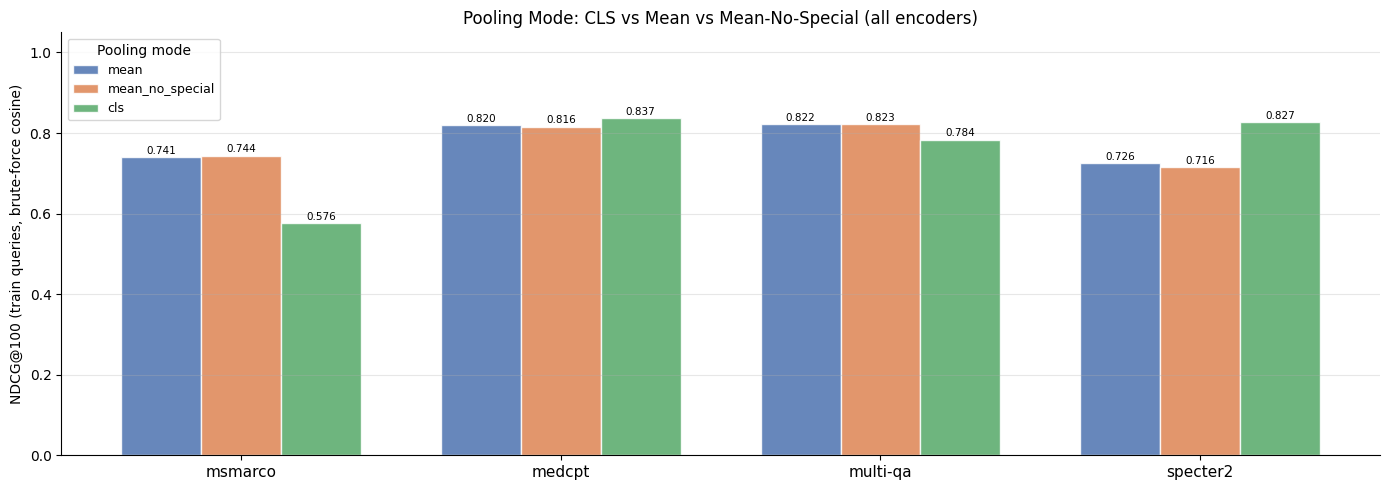
\includegraphics[width=\linewidth]{images/pooling_mode_sweep.png}
  \caption{Pooling-mode comparison --- NDCG@100 for each encoder $\times$
           pooling mode (brute-force exact cosine on 32 train topics).
           MedCPT + CLS yields the highest single score (0.8374).}
  \label{fig:pooling}
\end{figure}

\paragraph{Hybrid fusion:}
\textbf{Reciprocal Rank Fusion (RRF)}~\cite{rrf2009} merges two ranked lists
in a score-agnostic manner:
$\text{RRF}(d)=\sum_r \frac{1}{k + \text{rank}_r(d)}$, with $k$\,=\,60.
We fuse BM25 with KNN\,(MedCPT), chosen because lexical and semantic
signals are largely complementary.

%%%%%%%%%%%%%%%%%%%%%%%%%%%%%%%%%%%%%%%%%%%%%%%%%
%%%%   SECTION 2b — LLM Augmented Generation %%%%
%%%%              (Phase 2)                  %%%%
%%%%%%%%%%%%%%%%%%%%%%%%%%%%%%%%%%%%%%%%%%%%%%%%%

\subsection{LLM Augmented Generation (Phase~2)}
\label{sec:phase2}
\subsubsection{Exercise}
Before proceeding with the development of the Retrieval-Augmented Generation system, we conducted three exercises to better understand how the positional and contextual embeddings, and self-attention as input embeddings go through the different layers.

\textbf{Positional Embeddings:} To analyze the structure of a BERT model's (MedCPT Query Encoder) positional embeddings, a sequence of 200 repetitions of the word "cat" was constructed and fed to the model. Since all tokens are identical (excluding CLS and SEP), the variation observed in the embeddings is only due to the differences in positional information related to where that token is in the input sentence (sequence information). For each token, the cosine distance to the first token was computed and illustrated in a graph with colour that encodes the distance value. As seen in the left of the Figure~\ref{fig:exercise_distances} below, the distance increases with token position, confirming that BERT's positional embeddings encode sequential order in a geometrically consistent manner, meaning that tokens that are closer in position are also closer in positional embedding space in a consistent way.

\begin{figure}[htbp]
  \centering
  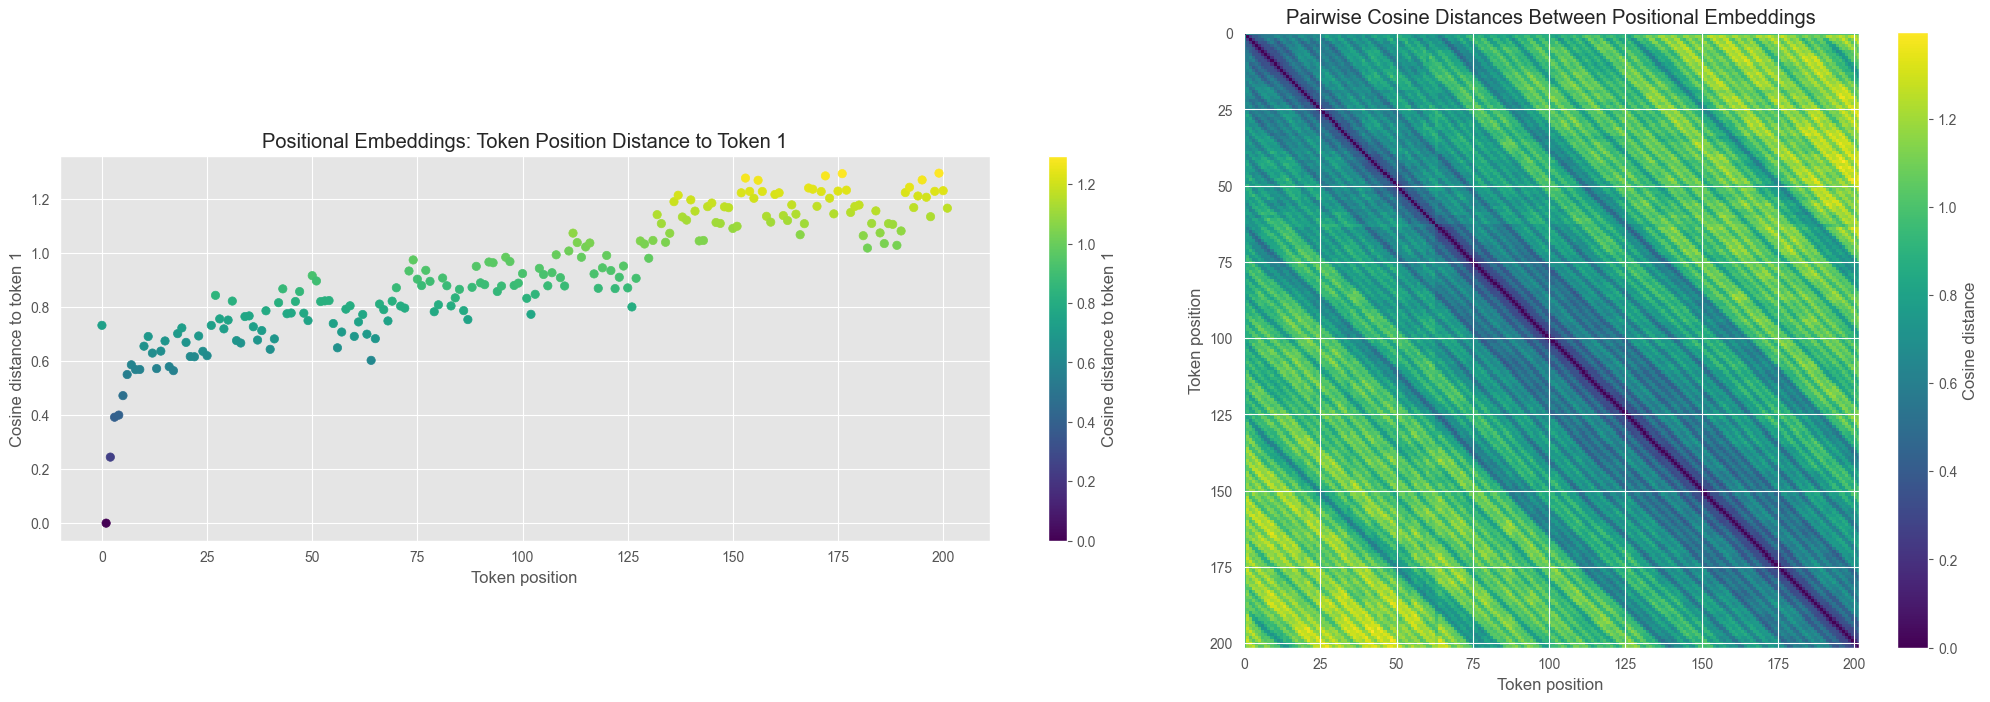
\includegraphics[width=\linewidth]{images/exercise_distances.png}
  \caption{Left: positional embeddings distances to the first "cat" token; Right: pairwise cosine distances between all tokens' positional embeddings}
  \label{fig:exercise_distances}
\end{figure}

Note that the CLS token has a cosine distance of 0.73 to the first token, which is normal since it is always fixed in position 0, due to the model also needing to learn a learn positional embedding for it. Its function is to serve as a summary token used in classification tasks.

This behaviour is further corroborated by the pairwise cosine distance matrix in the right of the previous Figure, which displays the distances between all pairs of token positions. It shows us a clear diagonal structure where entries closer to the main diagonal correspond to tokens closest in position and show low cosine distances (darker colour), while off-diagonal entries grow progressively larger as the positional gap between both tokens increase. This "banded" pattern confirms that positional similarity decays smoothly with distance, and that BERT's positional embeddings preserve a notion of local neighbourhood where nearby positions remain geometrically proximate in the embedding space.

\textbf{Contextual Embeddings:} To study how BERT models build contextualized semantic representations across layers, we extracted the output hidden states from all 12 layers and projected them into 2D/3D spaces with PCA.
Using the sentence "The cell membrane contains receptors. The receptor binds the ligand. Ligand binding activates the cell signaling pathway.", we observed that, in early layers, token representations form relatively "mixed" clusters with limited semantic relation. By layer 5, related tokens like "binds" and "binding" remain closer to each other in the embedding space, and are also closer to "receptor" than to less related concepts like "membrane" or "pathway". This behaviour is consistent with biomedical semantics, as binding interactions can be associated to receptor activity. In the final layers (of which the last can be seen in 3D in the Figure~\ref{fig:exercise_contextual}), the semantic organization becomes evident: signaling/activation tokens are closely related, and interaction-related concepts such as bindings and receptor interactions occupy a separate semantic region. Notably, the 2D projection placed "membrane" misleadingly close to these groups; the 3D projection revealed it is actually distant from both roughly at near the same distance/similarity with the SEP and "the" tokens, highlighting the limitations of 2D (first two eigenvalues) PCA appearing almost as far from them as from the isolated SEP and "the" tokens. The usage of the only first two eigenvalues made us lose that information (in 2D). Overall, this confirmed BERT progressively transforms lexical information into higher-level biomedical semantic structure across its layers.

\begin{figure}
    \centering
    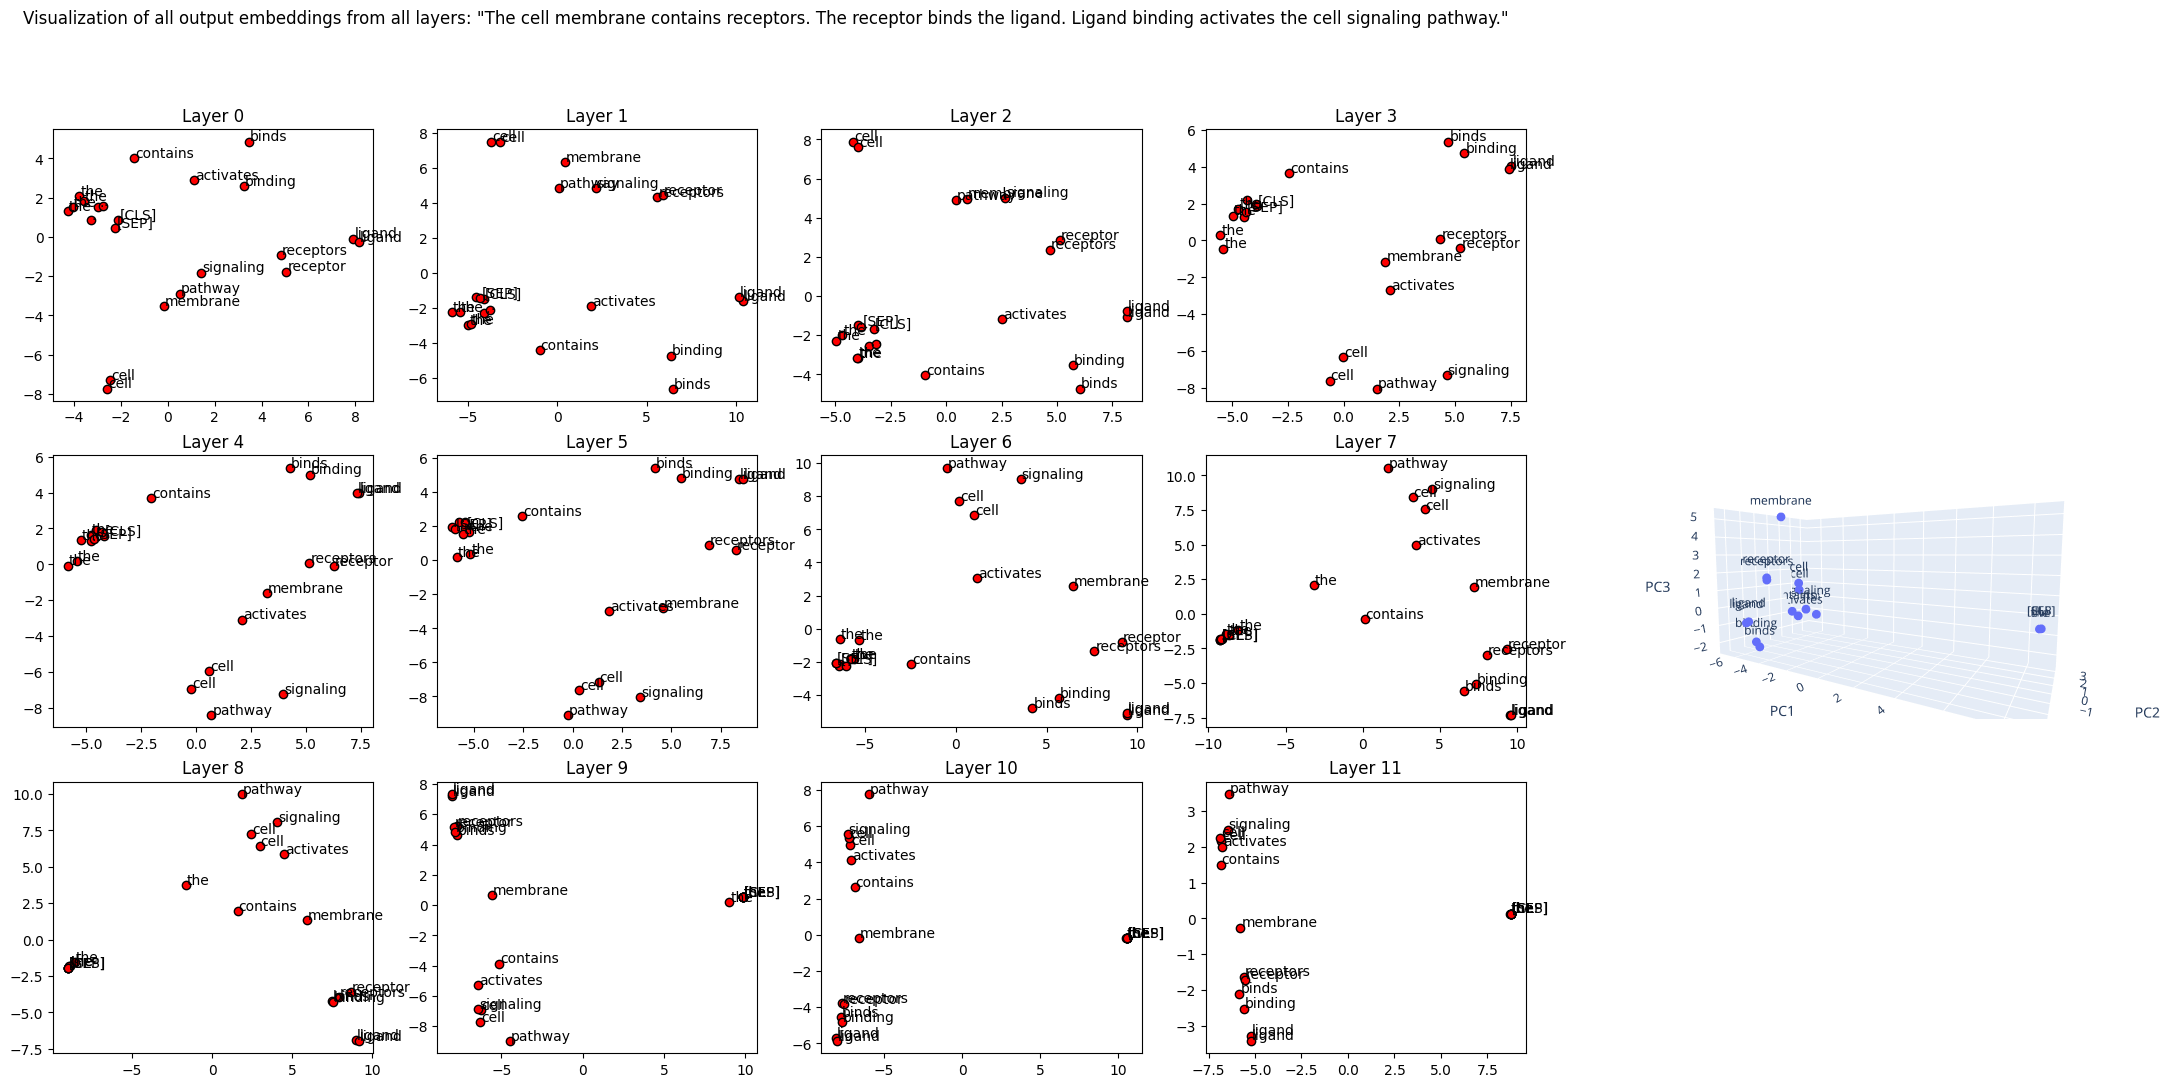
\includegraphics[width=\linewidth]{images/exercise_contextual.png}
    \caption{Left: 2D PCA projection of example contextual embeddings; Right: 3D PCA projection of example contextual embeddings}
    \label{fig:exercise_contextual}
\end{figure}

\textbf{Self-Attention:} For this exercise, we examined the self-attention mechanism of a transformer cross-encoder; in this case, MedCPT's Cross-Encoder.

One of the many examples we tested is the query "What drugs were prescribed to the patient with fever?" with answer "The patient was prescribed aspirin and ibuprofen to treat the fever.".

\begin{figure}
    \centering
    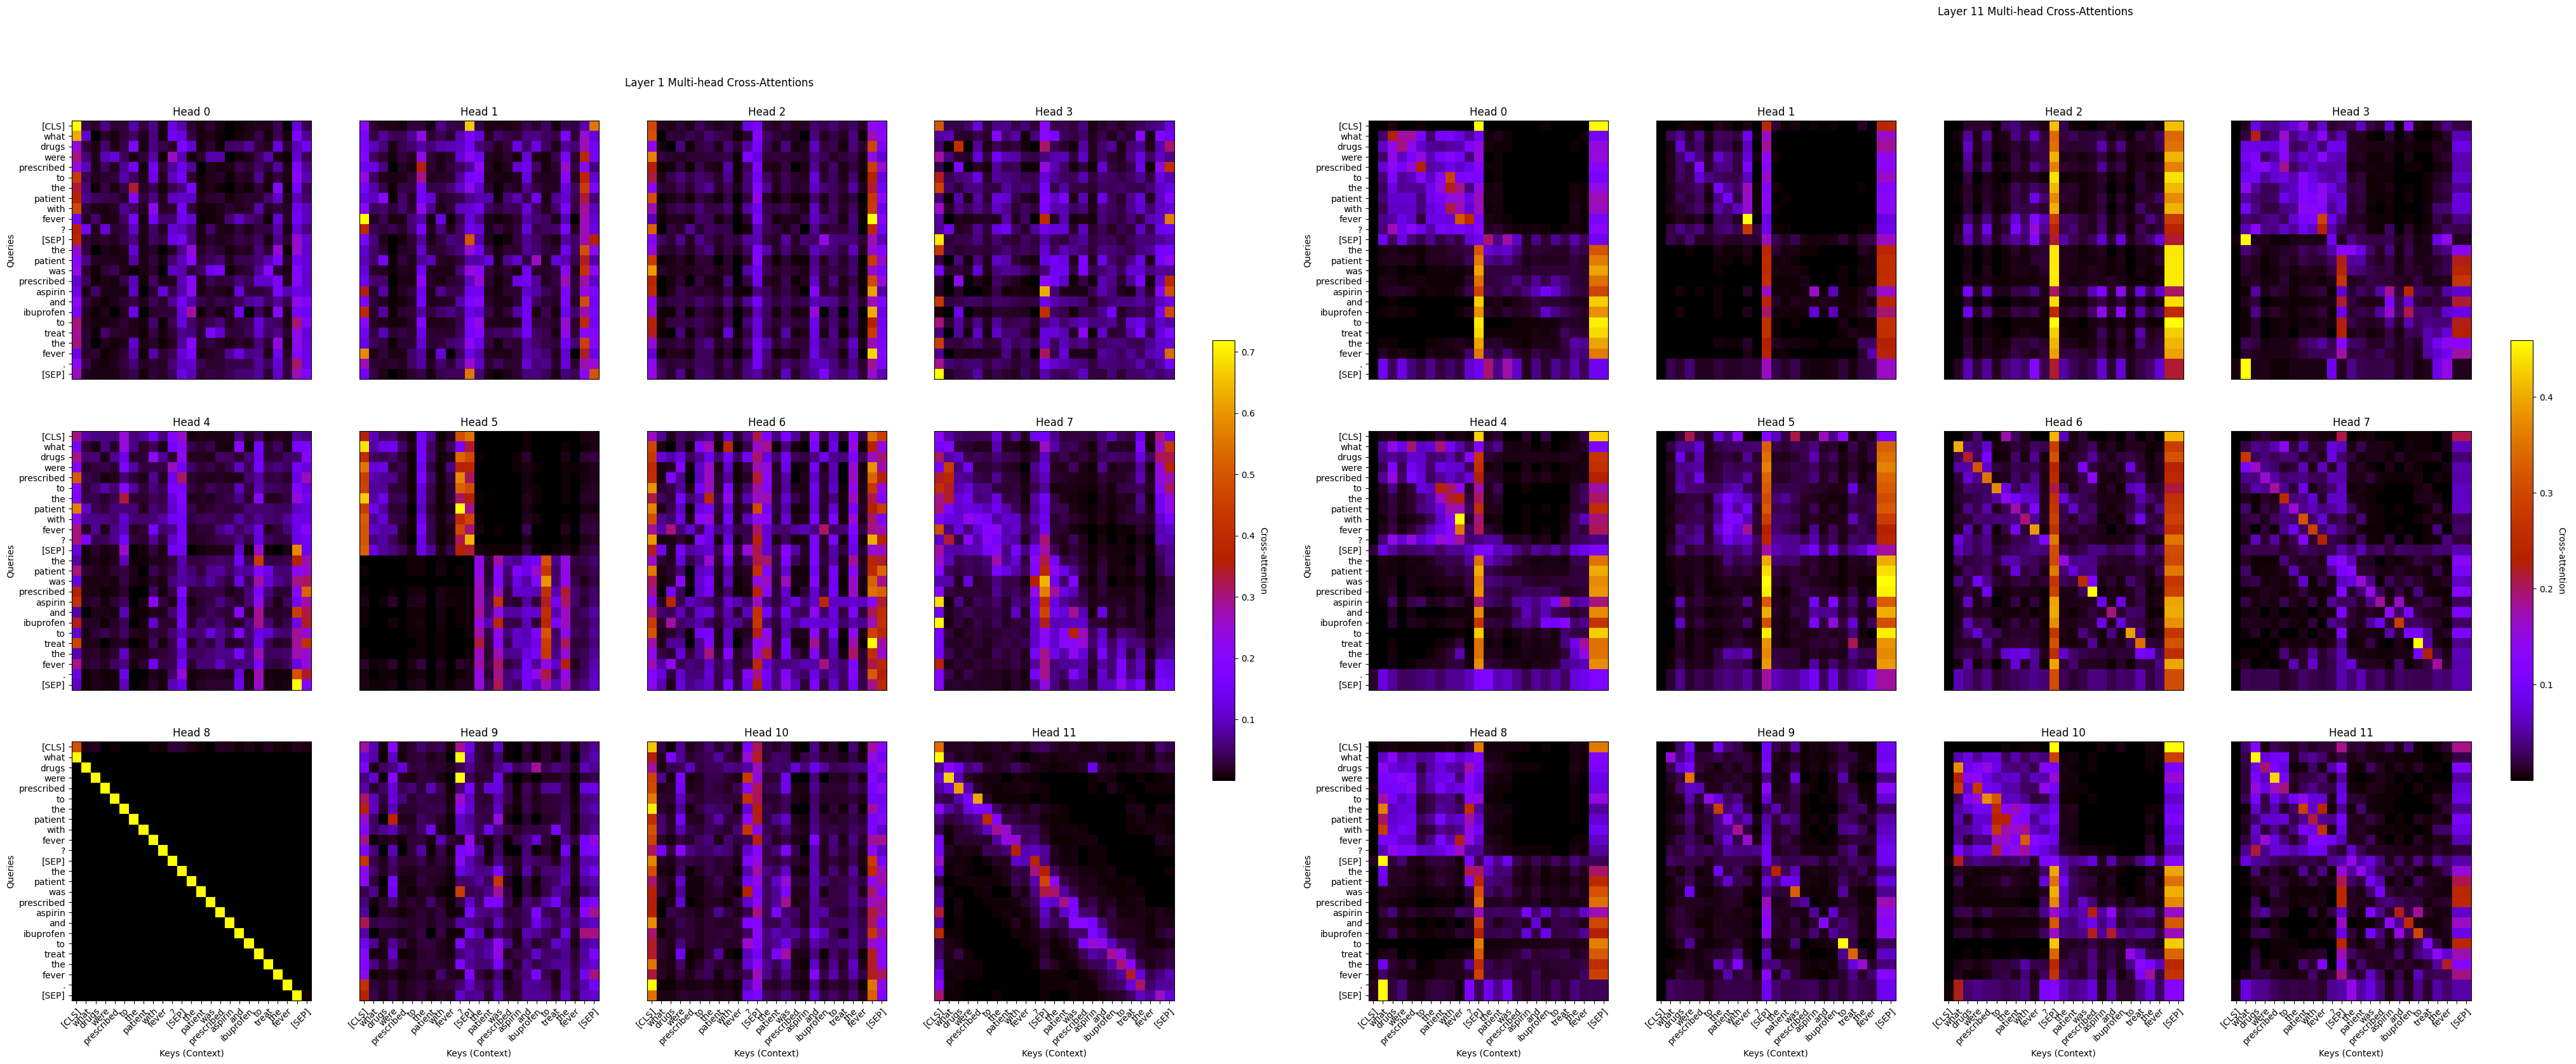
\includegraphics[width=\linewidth]{images/exercise_attention.png}
    \caption{Left: multi-head cross attentions for layer 1; Right: multi-head cross attentions for layer 11}
    \label{fig:exercise_attention}
\end{figure}

In this case, the layer one's attention heads tendentially focus more on local relations and basic syntatic dependencies, which can be seen in the high cross-attention values (brighter coloured) near the main diagonal of the matrices; these early attention heads tend to display more broad distributed attention. The final layer's attention heads attention values indicate a stronger and more specific cross-sentence attention; each head plays a specific, specialized role, allowing the model to better capture multiple perspectives on the input data. This is even more evident in the full visualization of all layers' multi-head self attentions in the Appendix~\ref{fig:model_view}.
Layer one shows a tendency of certain columns having a high attention score, but this is way more evident in the last layer, which illustrates the phenomenom of attention sink: the attention weights must sum to 1, but a token might not have a semantically meaningful target to attend to and it still has to place its probability mass somewhere; in this case, SEP becomes that "dump" token due to the fact that attending to it doesn't corrupt representations since its value vector is relatively uniformative, so routing attention there causes less damage than if it were done to other tokens.

\subsubsection{Answer Generation}
Phase 2 leverages the previous phase's results to extend the retrieval pipeline into a Retrieval-Augmented Generation system. To do this, we use MedCPT's Query Encoder to retrieve the index documents that best match a query, and then the Cross-Encoder reranker for sentence-level relevance scoring in order to get a well-built context to this specific query, that can be then passed to a decoder (Gemma 4 31B Instruction-Tuned) that generates a grounded answer with PMID citations.
Since the provided PubMed abstracts are plain text and are in the biomedical field, this requires a robust sentence boundary detection tool, rather than simple paragraph/period segmentation, in order to separate the abstracts into sentences. So, we analyzed (analytically) the difference between two different sentence segmentation libraries: NLTK and scispaCy.

\begin{table}[htbp]
\centering
\caption{NLTK vs. scispaCy comparison}
\label{tab:nltk_siscpacy}
\begin{tabular}{cccc}
  \hline
  \textbf{Property} & \textbf{NLTK} & \textbf{scispaCy} \\
  \hline
  Domain & General & Biomedical / Scientific Text \\
  Abbreviation Handling & Limited & Biomedical abbreviation-aware \\
  Basis & Statistics & Neural-Based \\
  Use Case & General NLP & Scientific Literature \\
  \hline
\end{tabular}
\end{table}

In theory, scispaCy should be much more appropriate for our use case, and this was also confirmed with the manual analysis of the sentence segmentation of 4 randomly selected corpus abstracts, and 1 handmade test. The handmade test is enough to understand why this sentence segmentation tool is the best choice (Fig.~\ref{fig:nltk_scispacy}):

\begin{figure}[htbp]
  \centering
  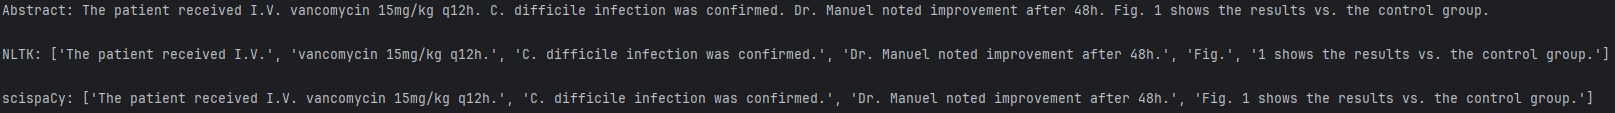
\includegraphics[width=\linewidth]{images/nltk_scispacy.png}
  \caption{NLTK vs. scispaCy: handmade test results}
  \label{fig:nltk_scispacy}
\end{figure}

scispaCy correctly identified abbreviations like "I.V." (intravenous) and preserved the sentence "The patient received I.V. vancomycin 15mg/kg q12h" as a single unit; NLTK incorrectly split it into two. This is critical when processing field-specific biomedical text like our dataset has. An additional example that further illustrate this difference is provided in the Appendix~\ref{fig:nltk_sciscpacy_ex2}.

After segmenting abstracts with sispaCy, we evaluated two sentence selection strategies over the top-10 retrieved documents (using MedCPT's Query Encoder). The first ranked all sentences from those documents by sorting the results of the MedCPT's Cross-Encoder, and then selected the top-10 sentences globally. The second enforced a per-document cap of 3 sentences before applying the same global top-10 selection.
Gemma 4 was then evaluated with a wide range of parameters (temperature, top-p, max sentences per document) and two different prompt templates using a frontier LLM as a Judge in order to identify the optimal setup for Phase 3. Varying the model parameters (temperature and top-p) allowed us to balance the model's output randomness by reshaping the probability distributions over the vocabulary, and restricting the set of candidate tokens, allowing us to assess whether a greater determinism improves answer quality. The two user prompt templates, in turn, explore whether providing the model with the full query context, topic, question and narrative, gives better results than only providing the context and question.
%%%%%%%%%%%%%%%%%%%%%%%%%%%%%%%%%%%%%%%%%%%%%%%%%
%%%%  SECTION 2c — LLM Agentic Patterns      %%%%
%%%%              (Phase 3)                  %%%%
%%%%%%%%%%%%%%%%%%%%%%%%%%%%%%%%%%%%%%%%%%%%%%%%%

\subsection{LLM Agentic Patterns (Phase~3)}
\label{sec:phase3}

To be developed in future work.


%% Section 3: Evaluation
%%%%%%%%%%%%%%%%%%%%%%%%%%%%%%%%%%%%%%%%%%%%%%%%%
%%%%   SECTION 3a — Evaluation Setup         %%%%
%%%%   Datasets, Metrics & Protocols         %%%%
%%%%%%%%%%%%%%%%%%%%%%%%%%%%%%%%%%%%%%%%%%%%%%%%%

\section{Evaluation}
\label{sec:eval}

\subsection{Experimental Setup: Datasets, Metrics and Protocols}
\label{sec:eval_setup}

% ══════════════════════════════════════════════════════════════════════════════
% 3.1.1  PHASE 1
% ══════════════════════════════════════════════════════════════════════════════
\subsubsection{Phase 1: Retrieval Evaluation}

\paragraph{Datasets and Relevance Judgements:}
Our evaluation uses the TREC BioGen 2024 collection: 4{,}194 PubMed abstracts
and 65 biomedical topics (IDs~116--180).  Full corpus and topic details are
described in §\ref{sec:phase1}.

Relevance judgements are derived from
\texttt{biogen\_2024\_\allowbreak submissions.json} --- automated BioGen~2024 system
submissions with sentence-level citation assessments
(\texttt{evidence\_relation} field).
Evidence relation value counts:
supporting=10{,}240; neutral=1{,}412; not relevant=2{,}201;
contradicting=275; invalid citation=635.

We construct two relevance scales from this data.
\textbf{Binary qrels} (used for P@10, R@100, MAP, and MRR) assign score\,=\,1
when \texttt{evidence\_relation} equals \texttt{"supporting"} and 0~otherwise, yielding
2{,}999 relevant (topic, PMID) pairs across all 65~topics (mean 46.1 relevant
docs per topic, range 8--88; every topic has at least one relevant document).
\textbf{Graded qrels} (used for NDCG@100) map supporting$\to$5,
neutral$\to$2, and all others$\to$0, taking the maximum score per
(topic, PMID) pair.  This produces 3{,}217 graded pairs (mean 49.5 relevant
docs per topic), with 2{,}999 at score\,=\,5 and 218 at score\,=\,2.

Two caveats apply.  First, these judgements are citation-based from automated
systems, not from human assessors.  Second, the mean of 46.1 relevant documents
per topic is $3\text{--}15\times$ above standard TREC tasks, so MAP and recall
values are not directly comparable to published IR benchmarks.
Additionally, PMID~37711029 (topic~141) is absent from the filtered corpus
and is excluded with a logged warning; 11~further PMIDs appearing only in
neutral citations are also excluded.

\paragraph{Split Protocol and Cross-Validation:}
We adopt a fixed odd/even split on topic IDs (as mandated by the course
instructor): 32~train queries (odd IDs: 117, 119, \ldots, 179) and
33~test queries (even IDs: 116, 118, \ldots, 180).  The corpus is shared
across both sets --- only the query set is partitioned.

Hyperparameter selection follows a strict sequential protocol:
(1)~query field ablation using BM25 on the train set to lock the query field;
(2)~LM-JM $\lambda$ sweep on the train set with 5-fold CV;
(3)~BM25 $k_1$/$b$ grid sweep on the train set with 5-fold CV;
(4)~LM-Dir $\mu$ sweep on the train set with 5-fold CV;
(5)~dense encoder and pooling comparison on the train set via brute-force
exact cosine; and finally
(6)~a single evaluation of all locked strategies on the test set, with no
further tuning.

The 5-fold cross-validation over 32~train queries assigns roughly
26~queries to training and 6~to validation in each fold.
The primary selection criterion throughout is mean NDCG@100 across folds.

\paragraph{Metrics:}
All metrics are implemented from scratch
in \texttt{src/\allowbreak evaluation/\allowbreak metrics\allowbreak .py}
(plain Python + NumPy, no external IR library ---
following the Lab03 protocol).

\begin{itemize}
  \item \textbf{P@10} (Precision at rank~10, binary qrels) ---
        of the first 10 retrieved documents, how many are truly relevant?
        A high P@10 means the practitioner sees mostly useful references
        on the first results page without manual filtering.

  \item \textbf{R@100} (Recall at rank~100, binary qrels) ---
        of all relevant documents in the collection, how many appear in
        the top~100?  This is critical for Phase~2: any relevant study
        \emph{not} retrieved here is permanently lost to the generation
        stage.

  \item \textbf{PR Curves} --- 11-point interpolated precision--recall
        curves averaged across test queries (Lab03 pattern).  They
        visualise the precision--recall trade-off across rank thresholds;
        the area under each curve approximates Average Precision.

  \item \textbf{AP\,/\,MAP} (Average Precision / Mean Average Precision,
        binary qrels) --- $\text{AP}=\frac{1}{|\mathcal{R}|}\sum_{k=1}^{n}
        P(k)\cdot\text{rel}(k)$, averaged across queries to obtain MAP.
        AP rewards systems that rank relevant documents near the top,
        not merely retrieving them somewhere in the list.

  \item \textbf{MRR} (Mean Reciprocal Rank, binary qrels) ---
        $\text{MRR}=\frac{1}{|Q|}\sum_{q}\frac{1}{\text{rank}_q^{(1)}}$.
        How quickly does the user find the \emph{first} useful result?
        MRR\,=\,1.0 means the top-ranked document is always relevant.

  \item \textbf{NDCG@100} (Normalised Discounted Cumulative Gain, graded
        qrels) --- the \textbf{primary TREC BioGen metric}:
        $\text{DCG}=\sum_{i=1}^{100}\frac{2^{\text{rel}_i}-1}{\log_2(i+2)}$;\;
        $\text{NDCG}=\text{DCG}/\text{IDCG}$.
        Unlike binary metrics, NDCG distinguishes \emph{how} relevant a
        document is (supporting\,=\,5 vs.\ neutral\,=\,2) and penalises
        highly relevant documents placed at low ranks, making it the most
        comprehensive single number for model selection.
\end{itemize}

% ══════════════════════════════════════════════════════════════════════════════
% 3.1.2  PHASE 2
% ══════════════════════════════════════════════════════════════════════════════
\subsubsection{Phase 2: Generation Evaluation}
To be developed in future work.

% ══════════════════════════════════════════════════════════════════════════════
% 3.1.3  PHASE 3
% ══════════════════════════════════════════════════════════════════════════════
\subsubsection{Phase 3: Agentic Evaluation}
To be developed in future work.

%%%%%%%%%%%%%%%%%%%%%%%%%%%%%%%%%%%%%%%%%%%%%%%%%
%%%%   SECTION 3b — Results and Discussion   %%%%
%%%%%%%%%%%%%%%%%%%%%%%%%%%%%%%%%%%%%%%%%%%%%%%%%

\subsection{Results and Discussion}
\label{sec:eval_results}

% ── 3b.1  QUERY FIELD ABLATION ────────────────────────────────────────────────
\subsubsection{Query Field Ablation (BM25, Train Set)}

The first step selects the query formulation.  Six combinations of the topic
fields were tested on 32 train queries using BM25 with default parameters as
the proxy retriever.  Table~\ref{tab:ablation} and
Figure~\ref{fig:field_ablation} show the results.

\textbf{Winner: \texttt{topic+question}} — NDCG@100=0.7833, MAP=0.5843.
The \texttt{narrative} field adds noise (instructions and qualifiers not found
in abstracts); \texttt{topic} alone misses clinical context synonyms.
The \texttt{topic+question} concatenation is locked for all subsequent
experiments.

\begin{table}[htbp]
\centering
\caption{Query field ablation — BM25 default on 32 train topics.
         Bold = winner; NDCG@100 is the selection criterion.}
\label{tab:ablation}
\begin{tabular}{lcccc}
  \hline
  \textbf{Field} & \textbf{NDCG@100} & \textbf{MAP} & \textbf{MRR}
                 & \textbf{P@10} \\
  \hline
  topic only       & 0.7381 & 0.5334 & \textbf{0.8255} & 0.6313 \\
  question only    & 0.7174 & 0.4988 & 0.8135 & 0.6562 \\
  narrative only   & 0.6099 & 0.3900 & 0.6890 & 0.5500 \\
  \textbf{topic+question}   & \textbf{0.7833} & \textbf{0.5843} & 0.8229 & \textbf{0.7000} \\
  topic+narrative  & 0.7205 & 0.5145 & 0.7083 & 0.6500 \\
  all three        & 0.7611 & 0.5673 & 0.7240 & 0.7031 \\
  \hline
\end{tabular}
\end{table}

\begin{figure}[htbp]
  \centering
  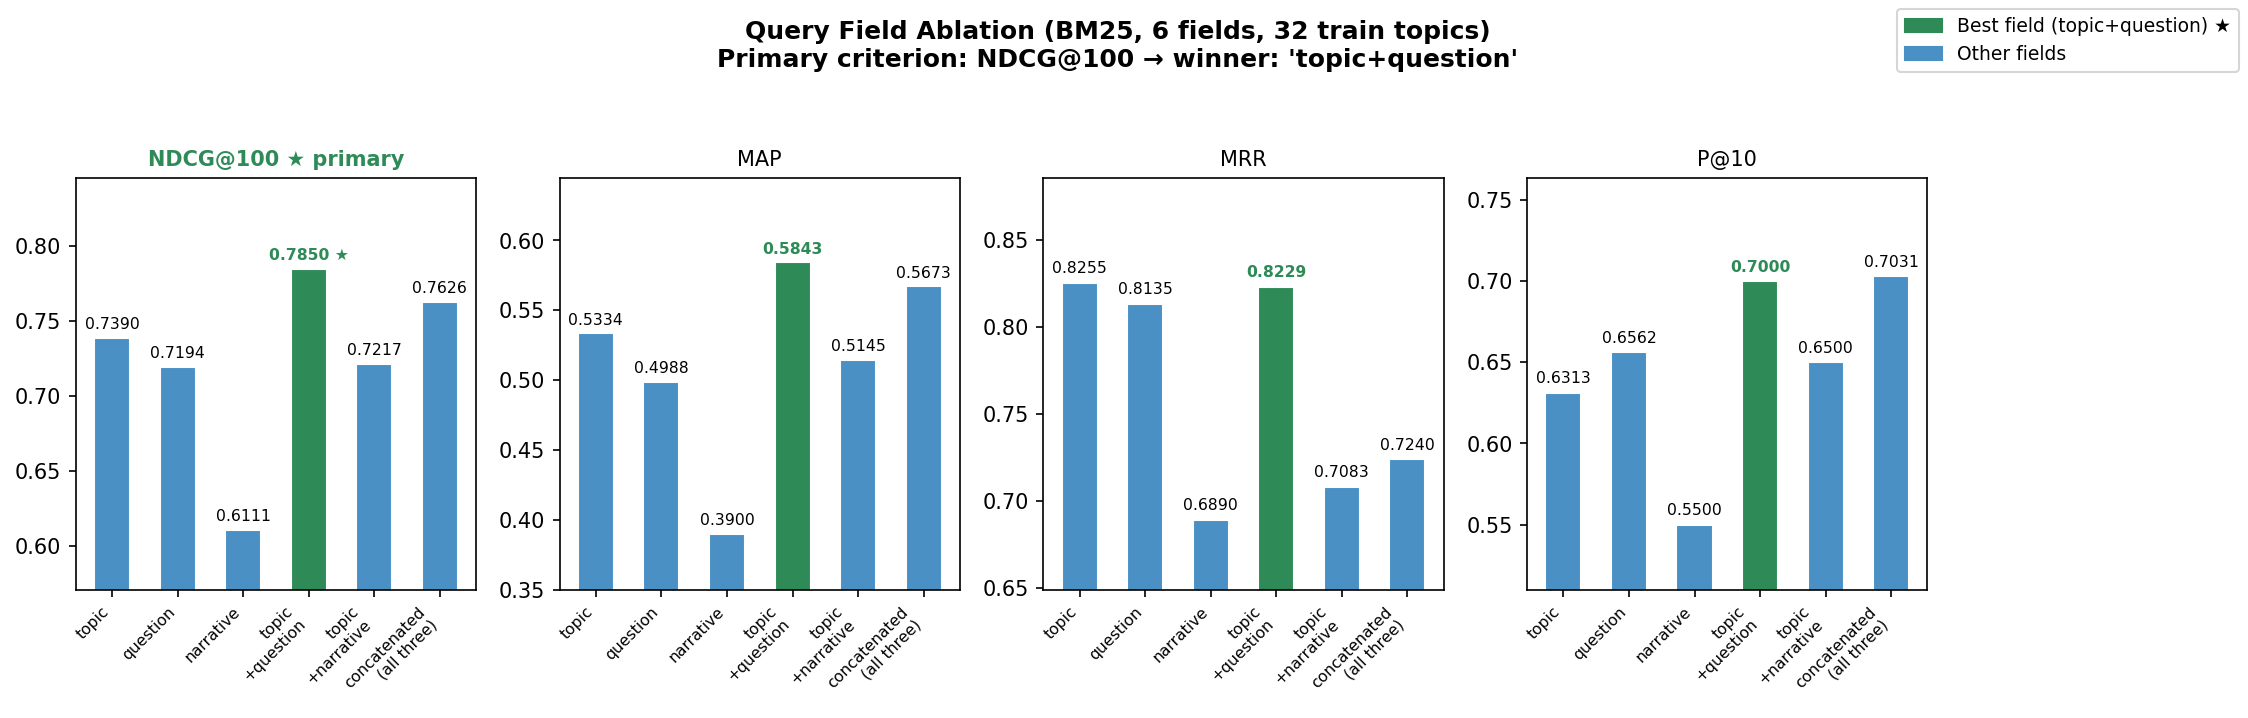
\includegraphics[width=\linewidth]{images/field_ablation.png}
  \caption{Field ablation results — NDCG@100 (primary) and MAP for each
           query formulation on the 32 train topics. \texttt{topic+question}
           achieves the highest NDCG@100 and is locked for all subsequent
           experiments.}
  \label{fig:field_ablation}
\end{figure}

% ── 3b.2  HYPERPARAMETER TUNING ───────────────────────────────────────────────
\subsubsection{Hyperparameter Tuning (5-Fold CV, Train Set)}

All sweeps use the locked \texttt{topic+question} field from
§\ref{sec:eval_setup}.

\paragraph{BM25:} $k_1 \times b$ grid, 24 configurations:
winner $k_1$=1.5, $b$=1.0 — NDCG@100=\textbf{0.7989}
($\Delta$=+0.0088 vs default $k_1$=1.2, $b$=0.75 at 0.7901).
High $b$=1.0 means full length normalisation: longer, more comprehensive
abstracts are rewarded rather than penalised.
See Figure~\ref{fig:bm25_sweep}.

\begin{figure}[htbp]
  \centering
  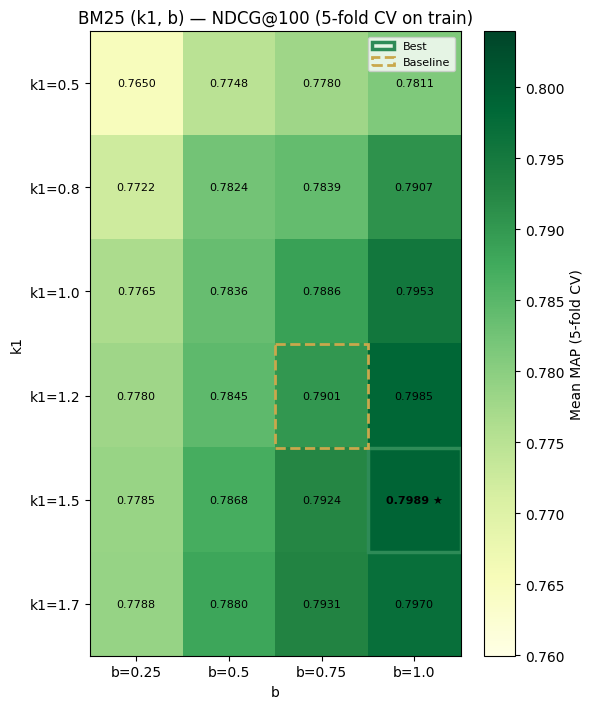
\includegraphics[width=0.70\linewidth]{images/bm25_param_sweep.png}
  \caption{BM25 $k_1$/$b$ sweep — mean CV NDCG@100. Winner: $k_1$=1.5,
           $b$=1.0.}
  \label{fig:bm25_sweep}
\end{figure}

\paragraph{LM Dirichlet:}
$\mu \in \{50, 75, 100, 125, 200, 500, 1000, 2000\}$:
CV winner $\mu = 100$ — NDCG@100 = 0.7706
($\Delta = {+}0.0196$ vs default $\mu = 2000$ at 0.7510).
The default $\mu$=2{,}000 is $\approx$13$\times$ the mean document length
(150~words) and over-smooths every abstract.
See Figure~\ref{fig:lmdir_sweep}.

\begin{figure}[htbp]
  \centering
  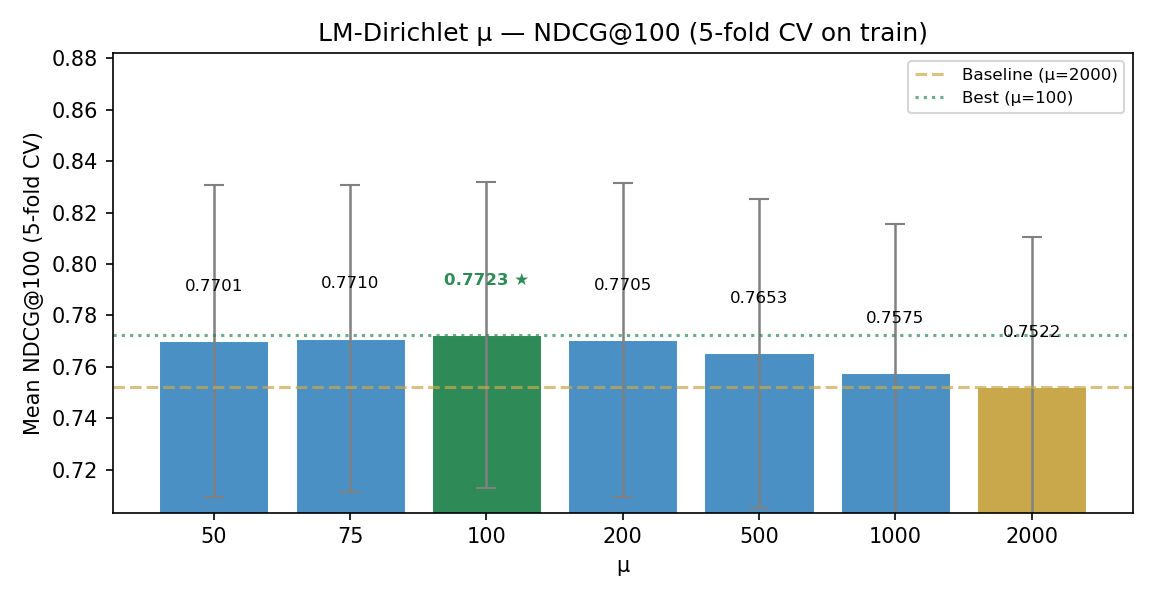
\includegraphics[width=0.92\linewidth]{images/lmdir_mu_sweep.png}
  \caption{LM-Dir $\mu$ sweep — mean CV NDCG@100. Default $\mu$=2000
           drastically under-performs; winner is $\mu$=100.}
  \label{fig:lmdir_sweep}
\end{figure}

\paragraph{LM Jelinek-Mercer:}
Seven values of $\lambda$ between 0.1 and 0.9 were tested (extended grid);
winner $\lambda = 0.65$ — NDCG@100 = 0.7754
($\lambda = 0.7$ at 0.7746; the extended grid confirms 0.65 edges ahead
by $\Delta = {+}0.0008$, within noise).
See Figure~\ref{fig:lmjm_sweep}.

\begin{figure}[htbp]
  \centering
  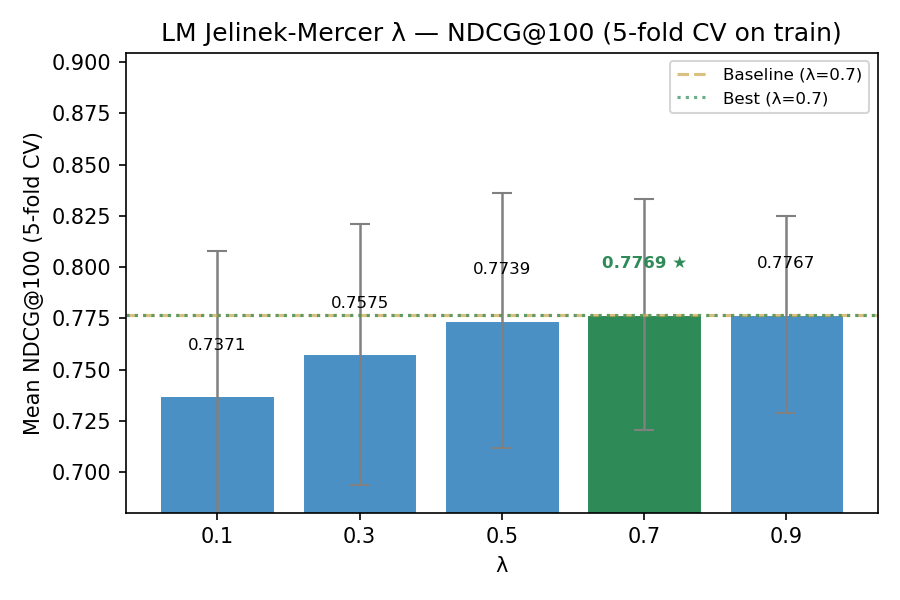
\includegraphics[width=0.82\linewidth]{images/lmjm_lambda_sweep.png}
  \caption{LM-JM $\lambda$ sweep — NDCG@100 plateaus in the 0.65--0.75 range;
           extended grid winner $\lambda$=0.65.}
  \label{fig:lmjm_sweep}
\end{figure}

\paragraph{Dense encoder comparison:}
MedCPT wins over multi-qa-mpnet, SPECTER-2, and
msmarco-distilbert — NDCG@100=\textbf{0.8273}
($\Delta$=+0.0825 vs msmarco baseline at 0.7448).
Trained on 23M PubMed click-through pairs, MedCPT is an exact domain match
for our task.  Encoder selection used brute-force exact cosine in Python
(not HNSW) to eliminate index-approximation noise; each encoder's best
pooling mode (CLS for MedCPT/SPECTER-2, mean-no-special for msmarco/multi-qa)
was determined first (see §\ref{sec:phase1}).
Full results are in Table~\ref{tab:encoder_comp} and
Figure~\ref{fig:encoder_sweep}.

\begin{table}[htbp]
\centering
\caption{Dense encoder comparison — 5-fold CV on 32 train topics (each
         encoder uses its best pooling mode from Table~\ref{tab:pooling}).
         Bold = best per column; $\star$ = selected encoder.
         MedCPT wins the primary metric (NDCG@100) despite multi-qa
         leading on MAP and P@10.}
\label{tab:encoder_comp}
\begin{tabular}{lcccc}
  \hline
  \textbf{Encoder} & \textbf{NDCG@100} & \textbf{MAP} & \textbf{MRR}
                   & \textbf{P@10} \\
  \hline
  MedCPT $\star$         & \textbf{0.8273} & 0.6209          & 0.8802          & 0.7094 \\
  multi-qa               & 0.8236          & \textbf{0.6435} & 0.8698          & \textbf{0.7719} \\
  msmarco (baseline)     & 0.7448          & 0.5403          & 0.8568          & 0.7469 \\
  SPECTER-2              & 0.7292          & 0.5177          & \textbf{0.8854} & 0.7500 \\
  \hline
\end{tabular}
\end{table}

\begin{figure}[htbp]
  \centering
  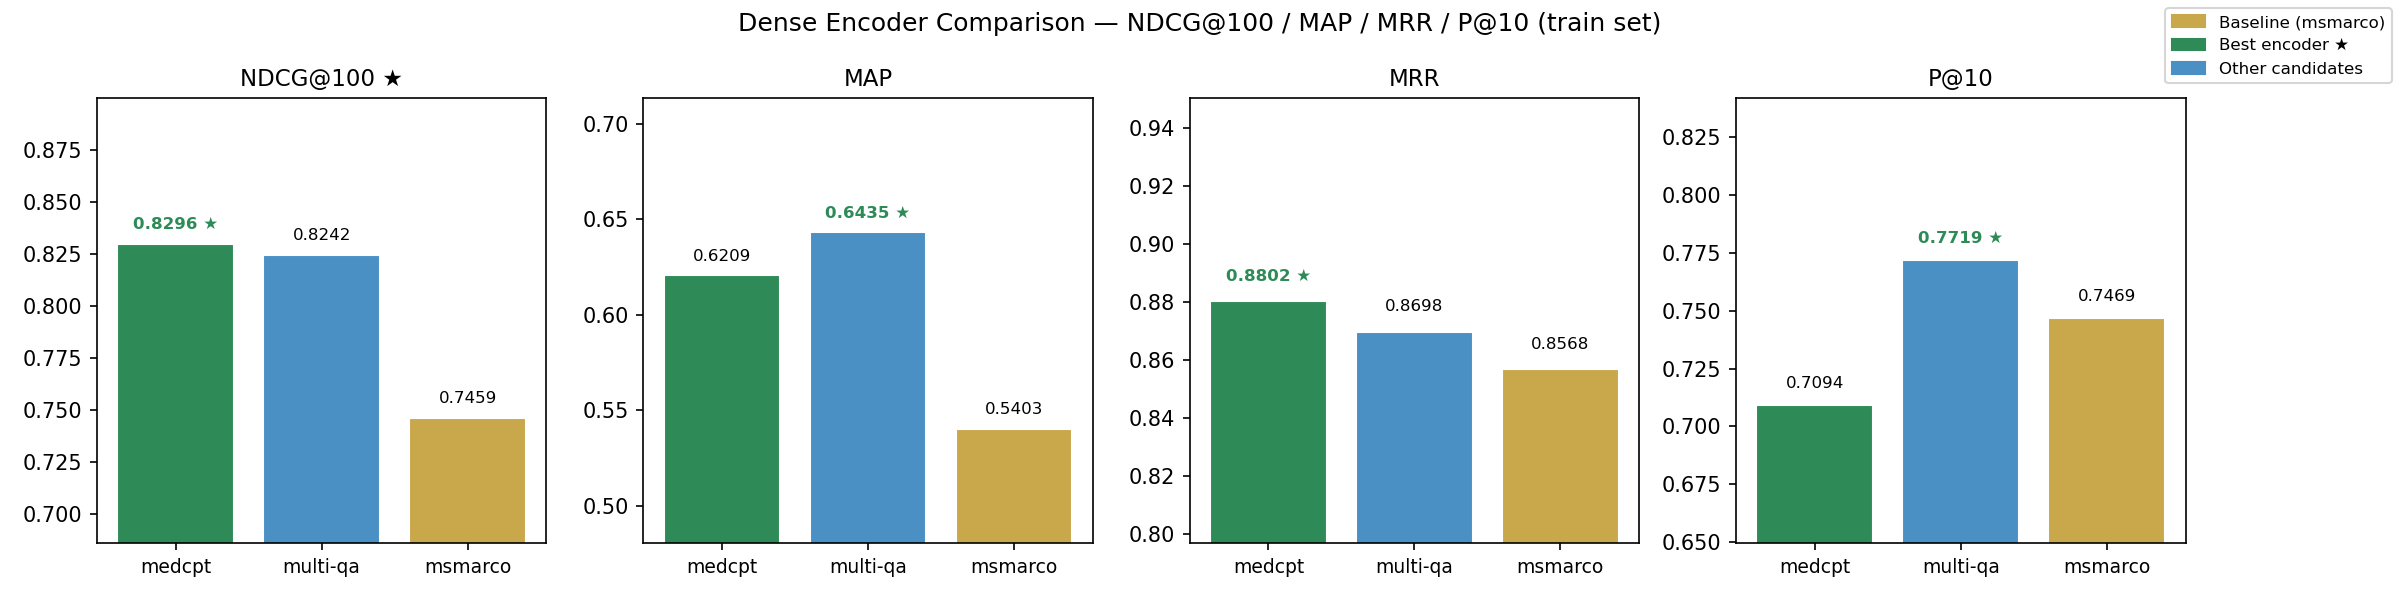
\includegraphics[width=\linewidth]{images/encoder_comparison.png}
  \caption{Encoder comparison — NDCG@100 on 32 train topics. MedCPT
           dominates (+0.0825 over msmarco baseline).}
  \label{fig:encoder_sweep}
\end{figure}

\paragraph{RRF pair sweep:}
Nine strategy pairs were tested across three $k$ values (30, 60, 90) in
5-fold CV.  The best lexical pair was BM25+LM-Dir at $k$=90
(NDCG@100=0.7907); however, no RRF pair surpasses KNN(MedCPT) solo
(0.8273) on the train CV leaderboard.
See Figure~\ref{fig:rrf_sweep}.

\begin{figure}[htbp]
  \centering
  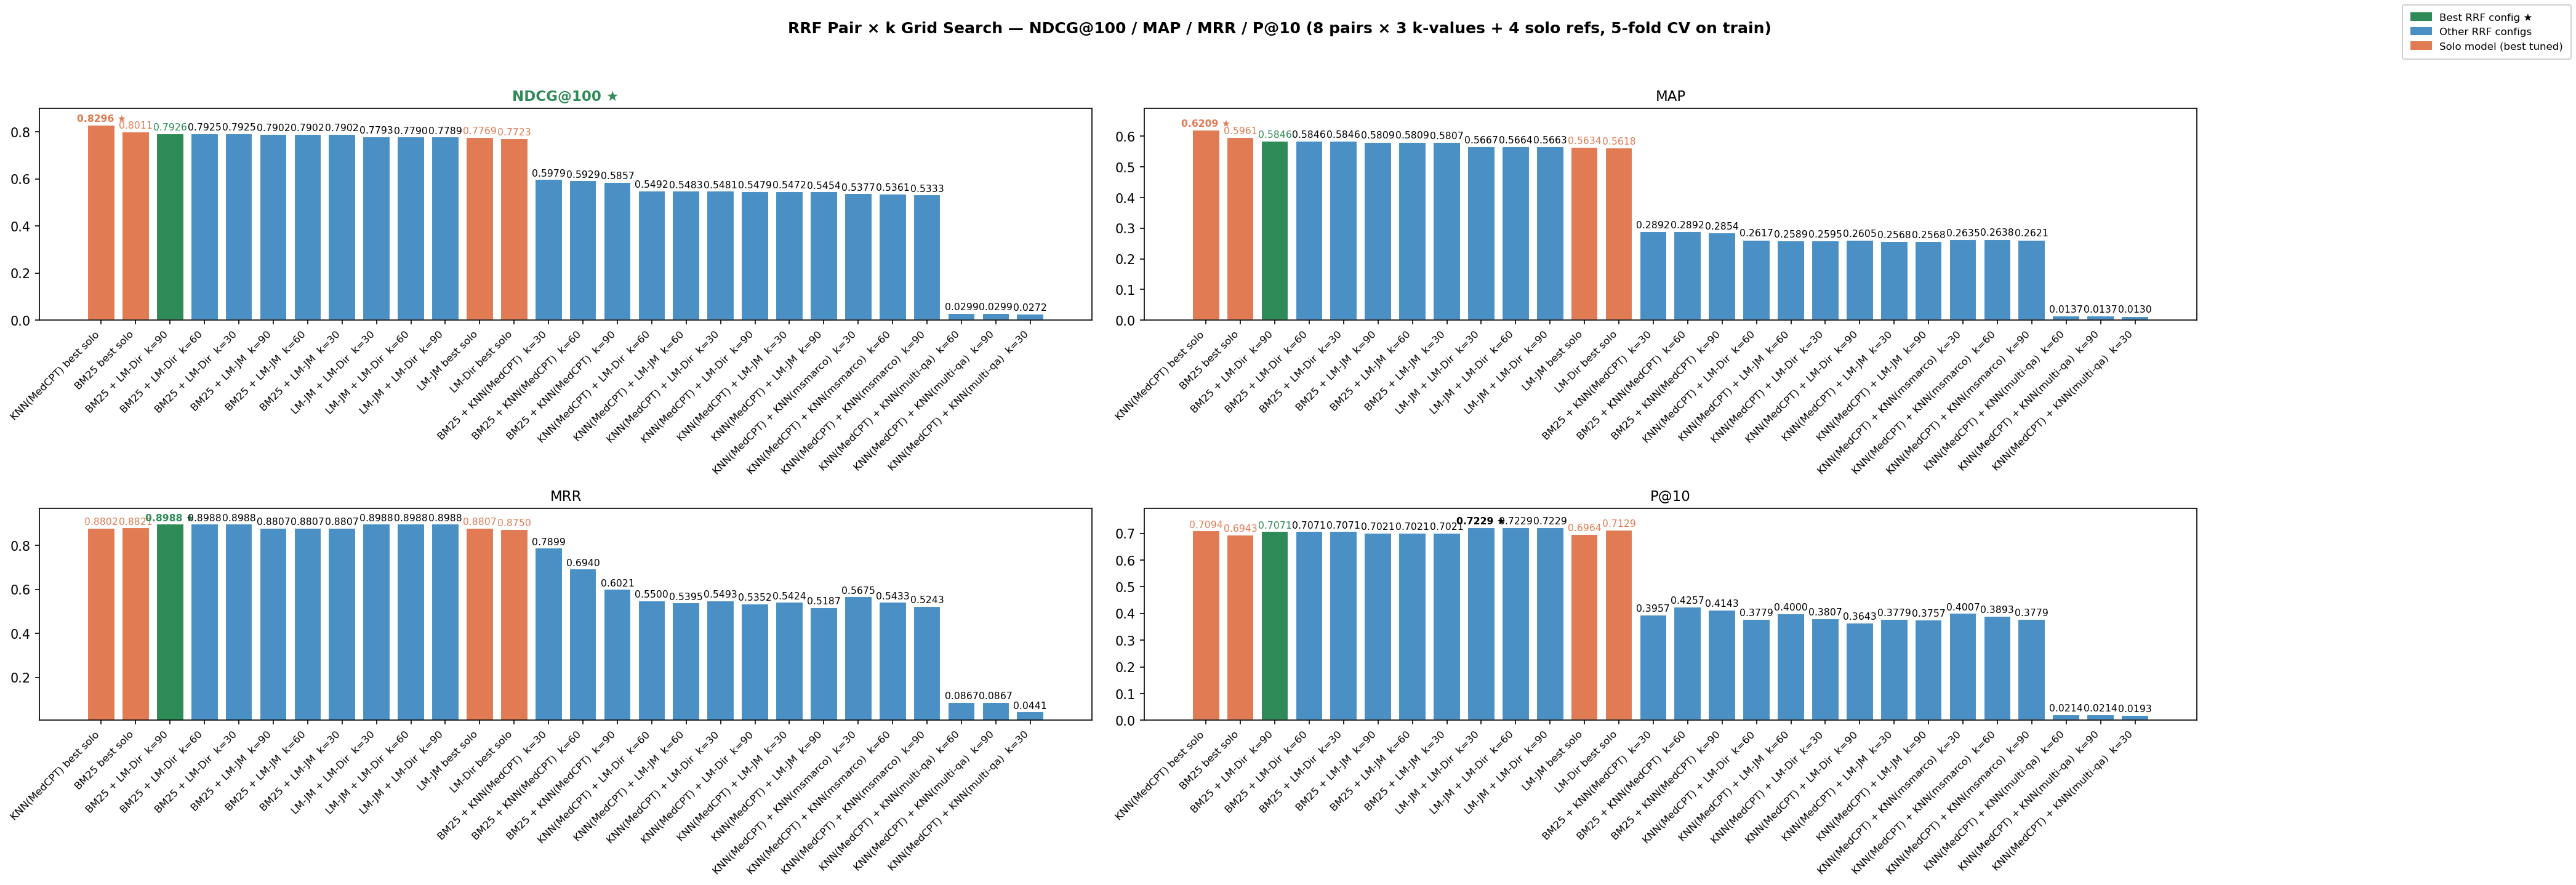
\includegraphics[width=\linewidth]{images/rrf_pair_sweep.png}
  \caption{RRF pair sweep — 9 strategy pairs $\times$ 3 $k$ values, 5-fold CV.
           Lexical pairs (BM25+LM-Dir, $k$=90, NDCG@100=0.7907) outperform
           KNN fusions at the rank-level.}
  \label{fig:rrf_sweep}
\end{figure}

\paragraph{Train CV summary:}
Table~\ref{tab:leaderboard} ranks all tuned strategies by NDCG@100
on the train CV; KNN(MedCPT) is the overall winner.
Figure~\ref{fig:tuning_summary} visualises the baseline-to-tuned gain for
each model; encoder selection (MedCPT) yields the largest gain,
followed by LM-Dir correction ($\mu = 100$).

\begin{table}[htbp]
\centering
\caption{Train CV leaderboard — all tuned solo strategies and the best RRF
         pair, ranked by NDCG@100 (5-fold CV on 32 train topics).
         KNN(MedCPT) is the overall winner; no RRF pair surpasses it.}
\label{tab:leaderboard}
\begin{tabular}{clcc}
  \hline
  \textbf{Rank} & \textbf{Strategy} & \textbf{NDCG@100} & \textbf{MAP} \\
  \hline
  1 & KNN (MedCPT)               & \textbf{0.8273} & \textbf{0.6209} \\
  2 & BM25 ($k_1$=1.5, $b$=1.0)  & 0.7989          & 0.5961 \\
  3 & RRF (BM25+LM-Dir, $k$=90)  & 0.7907          & 0.5846 \\
  4 & LM-JM ($\lambda$=0.65)     & 0.7754          & 0.5636 \\
  5 & LM-Dir ($\mu$=100)         & 0.7706          & 0.5618 \\
  \hline
\end{tabular}
\end{table}

\begin{figure}[htbp]
  \centering
  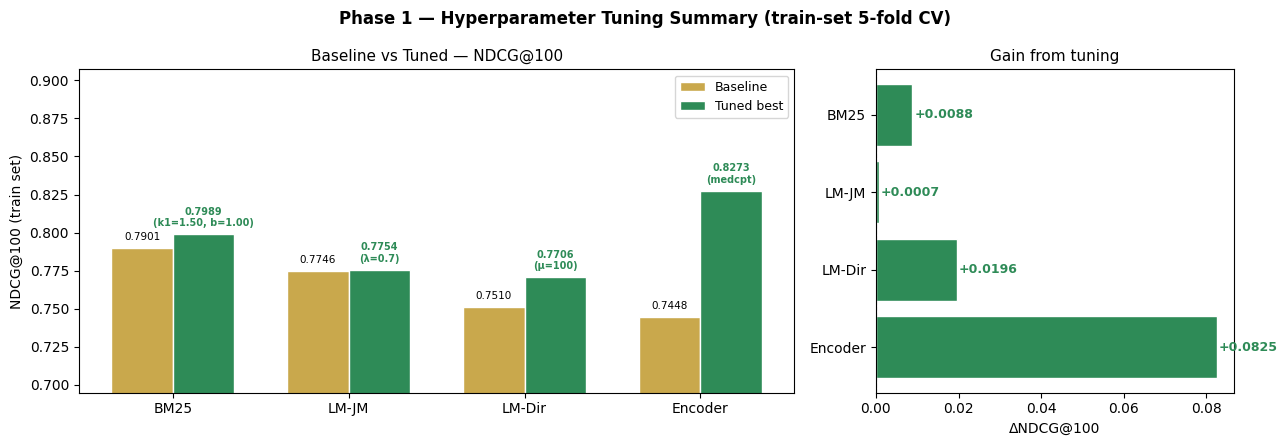
\includegraphics[width=\linewidth]{images/tuning_summary.png}
  \caption{Tuning summary: baseline vs.\ tuned NDCG@100 for every model
           (5-fold CV on 32 train topics). Encoder selection (MedCPT) yields
           the largest gain ($\Delta$NDCG@100=+0.0825 over msmarco); LM-Dir
           correction ($\mu$=100) yields the second-largest (+0.0196).}
  \label{fig:tuning_summary}
\end{figure}

% ── 3b.3  LOCKED CONFIGURATION ────────────────────────────────────────────────
\subsubsection{Locked Configuration}

All hyperparameters are locked after the train-set sweeps described above.
Table~\ref{tab:locked_config} lists the final configuration passed to
Phase~2.

\begin{table}[htbp]
\centering
\caption{Locked Phase~1 configuration.  All values selected on the 32-query
         train set (5-fold CV); test set touched once.}
\label{tab:locked_config}
\begin{tabular}{ll}
  \hline
  \textbf{Parameter} & \textbf{Value} \\
  \hline
  Query field               & \texttt{topic+question} \\
  BM25 $k_1$, $b$           & 1.5, 1.0 \quad (CV NDCG@100=0.7989) \\
  LM-JM $\lambda$           & 0.65 \quad (CV NDCG@100=0.7754) \\
  LM-Dir $\mu$              & 100 \quad (CV NDCG@100=0.7706) \\
  Dense encoder             & MedCPT (asymmetric, CLS pooling) \\
  RRF pair                  & BM25 + KNN(MedCPT), $k$=60 \\
  Best overall (train CV)   & KNN(MedCPT) — NDCG@100=0.8273 \\
  Best overall (test)       & RRF (BM25+MedCPT) — NDCG@100=0.8245 \\
  \hline
\end{tabular}
\end{table}

% ── 3b.4  TEST SET RESULTS ────────────────────────────────────────────────────
\subsubsection{Test Set Results (33 Topics)}

All strategies are evaluated once on the held-out test set after all
parameters are locked.  All use \texttt{topic+question}; top-100 results
per query.  Table~\ref{tab:test_results} compares baseline (default
parameters) against tuned configurations across all five metrics.
Figure~\ref{fig:tuning_gain} shows the per-strategy tuning gain.

\begin{table}[htbp]
\centering
\caption{Baseline (default parameters) vs tuned — all 5 metrics on the
         33-query test set. NDCG@100 is the primary metric (graded qrels).
         Bold = best per column.}
\label{tab:test_results}
\begin{tabular}{lccccc}
  \hline
  \textbf{Strategy} & \textbf{NDCG@100} & \textbf{MAP} & \textbf{MRR}
                    & \textbf{P@10} & \textbf{R@100} \\
  \hline
  \multicolumn{6}{l}{\textit{Baseline (default parameters)}} \\
  BM25 ($k_1$=1.2, $b$=0.75)   & 0.7756 & 0.5695 & 0.7712 & 0.6333 & 0.8594 \\
  LM-JM ($\lambda$=0.7)         & 0.7586 & 0.5431 & 0.7848 & 0.6333 & 0.8303 \\
  LM-Dir ($\mu$=2000)           & 0.7341 & 0.5149 & 0.7740 & 0.6212 & 0.8100 \\
  KNN (msmarco)                 & 0.7576 & 0.5561 & 0.8384 & \textbf{0.6879} & 0.8933 \\
  RRF (default)                 & 0.8114 & 0.6100 & 0.8141 & 0.6667 & 0.8921 \\
  \hline
  \multicolumn{6}{l}{\textit{Tuned (locked parameters)}} \\
  BM25 ($k_1$=1.5, $b$=1.0)    & 0.7742 & 0.5677 & 0.7141 & 0.6333 & 0.8600 \\
  LM-JM ($\lambda$=0.65)        & 0.7569 & 0.5413 & 0.7864 & 0.6212 & 0.8303 \\
  LM-Dir ($\mu$=100)            & 0.7555 & 0.5428 & 0.7773 & 0.6061 & 0.8270 \\
  \textbf{KNN (MedCPT)}         & 0.8077 & 0.6143 & 0.8000 & 0.6788 & \textbf{0.8933} \\
  \textbf{RRF (BM25+MedCPT)}   & \textbf{0.8245} & \textbf{0.6266}
                                & \textbf{0.8394} & 0.6515 & \textbf{0.9142} \\
  \hline
\end{tabular}
\smallskip\par\noindent\small
KNN(MedCPT) is the \emph{train CV winner} (NDCG@100=0.8273).
RRF (BM25+MedCPT, $k$=60) achieves the highest \emph{test-set} NDCG@100=0.8245.
\end{table}

\begin{figure}[htbp]
  \centering
  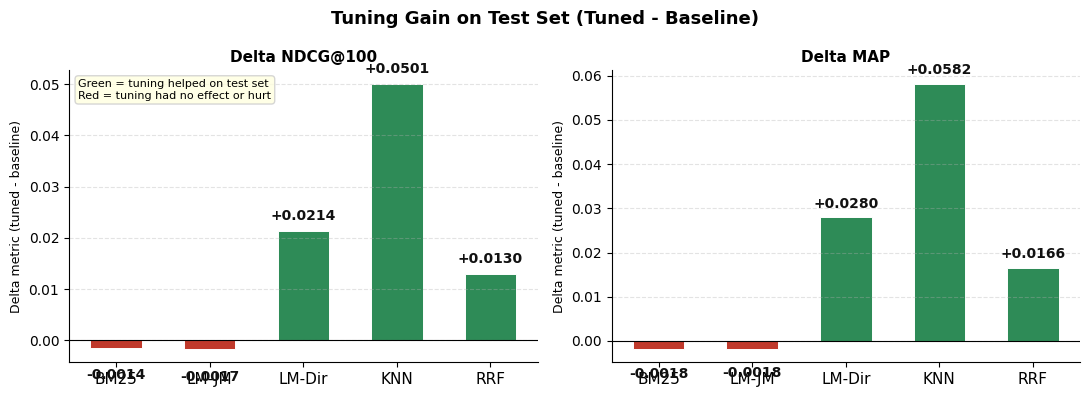
\includegraphics[width=\linewidth]{images/tuning_gain_test.png}
  \caption{Tuning gain on the test set ($\Delta$NDCG@100 and $\Delta$MAP,
           tuned $-$ baseline). KNN and RRF gain significantly; BM25 tuning
           yields no measurable gain ($\Delta$NDCG@100\,=\,$-$0.0014).}
  \label{fig:tuning_gain}
\end{figure}

\paragraph{Key observations:}
KNN\,(MedCPT) wins on the train CV
(NDCG@100 = 0.8273) and achieves
NDCG@100 = 0.8077, MAP = 0.6143, R@100 = 0.8933
on the test set, making it the locked Phase~2 backbone.
RRF (BM25 + MedCPT, $k = 60$) pushes the test NDCG@100 further to
0.8245 by fusing complementary lexical and dense signals.
Selecting MedCPT is the single most impactful change overall:
$\Delta$NDCG@100 = +0.0501 versus the msmarco KNN baseline on test
($0.7576 \to 0.8077$).
By contrast, BM25 tuning has minimal effect
($\Delta = -0.0014$ on test — tuning slightly hurt generalisation),
while LM-Dir tuning delivers a clear improvement
($\mu = 100$ versus $\mu = 2{,}000$: $0.7341 \to 0.7555$, +0.0214).
The R@100 of 0.8933 for KNN\,(MedCPT) covers more than 89\% of relevant
documents, providing a strong evidence pool for Phase~2 generation.

% ── 3b.5  PER-TOPIC ANALYSIS ─────────────────────────────────────────────────
\subsubsection{Per-Topic Analysis}

AP ranges widely across topics, revealing high sensitivity to query phrasing
and topic specificity.  Figure~\ref{fig:individual_pr} shows per-topic
PR curves for KNN\,(MedCPT), the locked Phase~2 strategy.
The best-performing topic is~170 (isoniazid hepatotoxicity,
AP\,=\,0.8961), whose specific clinical and drug terminology aligns well
with PubMed vocabulary.
The median case is topic~120 (causes of facial numbness, AP\,=\,0.6277),
while the hardest is topic~140 (spontaneous hand fractures, AP\,=\,0.1168),
where the broad, ambiguous query leaves few relevant PMIDs recoverable in
the top~100.
An informal IDF analysis suggests that low-IDF terms such as ``treatment''
and ``patient'' correlate with low AP, whereas disease-specific or
drug/gene-symbol terms tend to produce higher scores.

\begin{figure}[htbp]
  \centering
  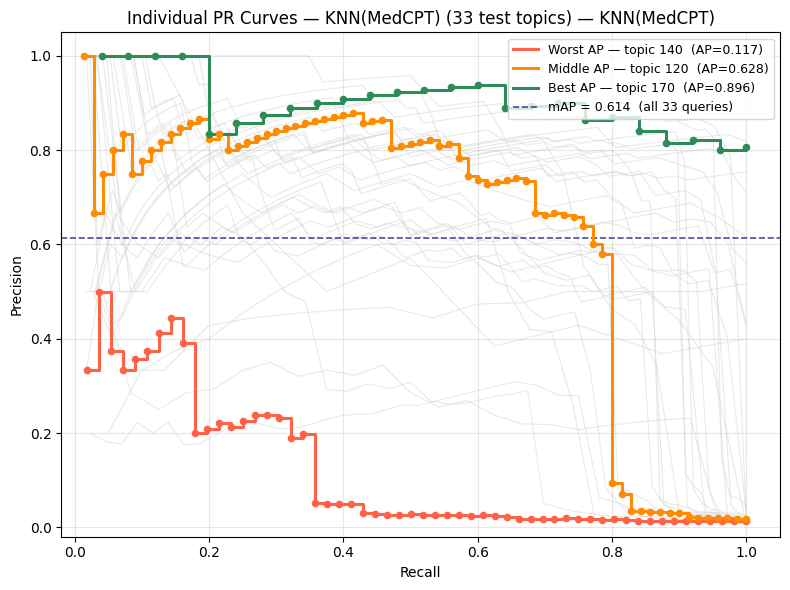
\includegraphics[width=0.85\linewidth]{images/individual_pr_curves.png}
  \caption{Per-topic PR curves for KNN(MedCPT) on all 33 test topics.
           Green = best topic (170 — isoniazid hepatotoxicity, AP=0.8961);
           red = worst topic (140 — spontaneous hand fractures, AP=0.1168);
           orange = median topic (120 — causes of facial numbness, AP=0.6277).
           Gray curves = remaining 30 topics.
           Dashed navy = mean AP (MAP=0.6143).
           Wide spread indicates high sensitivity to topic vocabulary.}
  \label{fig:individual_pr}
\end{figure}

Figure~\ref{fig:ap_boxplot} shows the AP distribution across all strategies.
RRF (tuned) achieves the highest median AP and the least variance, confirming
its robustness.  Note that the median AP for KNN(MedCPT) is slightly lower
than for RRF(tuned) because RRF fuses complementary lexical and dense
signals: BM25 rescues topics where the dense encoder struggles with
out-of-vocabulary biomedical terms, raising the floor AP.

\begin{figure}[htbp]
  \centering
  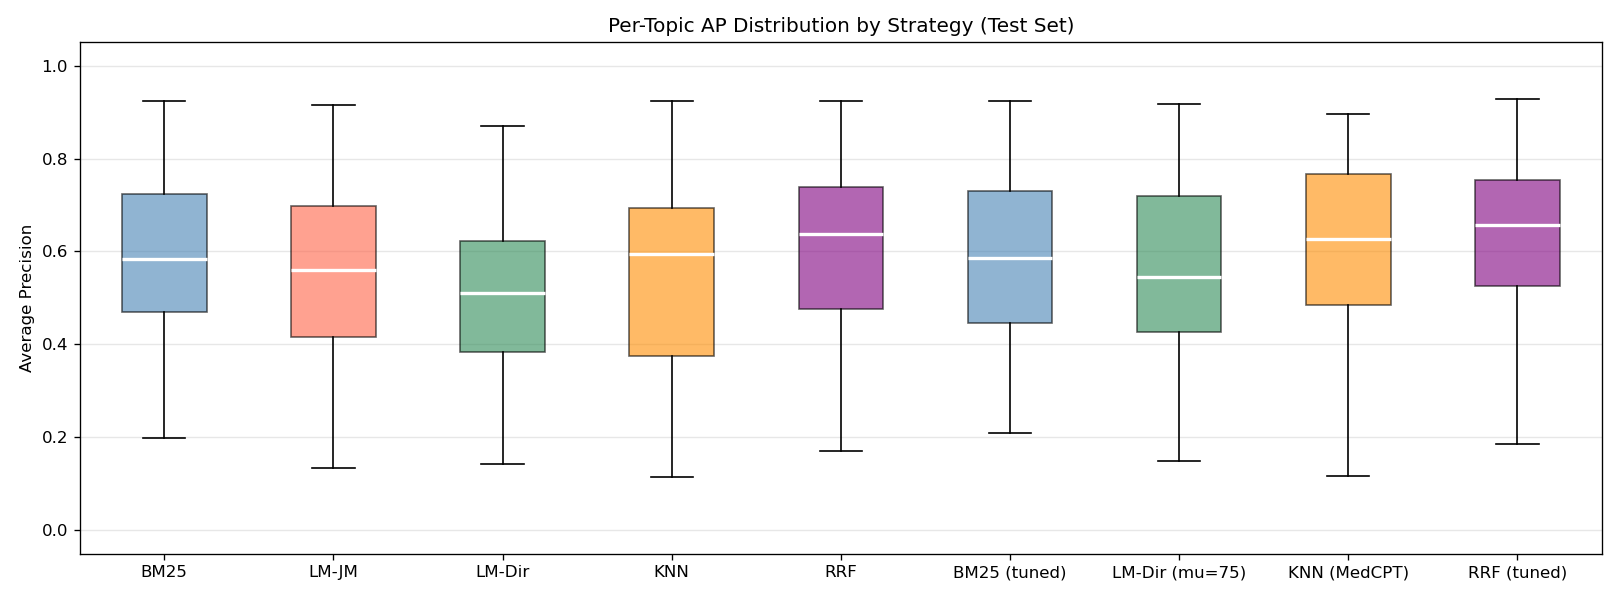
\includegraphics[width=0.80\linewidth]{images/ap_boxplot.png}
  \caption{Per-topic AP distribution across all strategies (test set, 33
           topics). RRF (tuned) achieves the highest median AP and the least
           variance. Wide IQR reflects inherent topic-difficulty spread.
           Outliers below the whisker correspond to hard topics (AP$<$0.3).}
  \label{fig:ap_boxplot}
\end{figure}

% ── 3b.6  PRECISION-RECALL ANALYSIS ──────────────────────────────────────────
\subsubsection{Precision-Recall Analysis (MAP)}

PR curves are computed as 11-point interpolated means across all 33 test
topics (Lab03 protocol).  The area under each curve approximates MAP —
a larger area indicates better overall ranking quality.

Figure~\ref{fig:pr_curves} shows the mean interpolated PR curves for all
strategies.  RRF (tuned) and KNN(MedCPT) dominate across the full recall
range.  The lexical LM variants show steeper early-recall drops, reflecting
their weaker semantic matching.  At high recall levels ($>$0.6), RRF
maintains notably higher precision than any single model, again illustrating
the benefit of fusing complementary retrieval signals.

\begin{figure}[htbp]
  \centering
  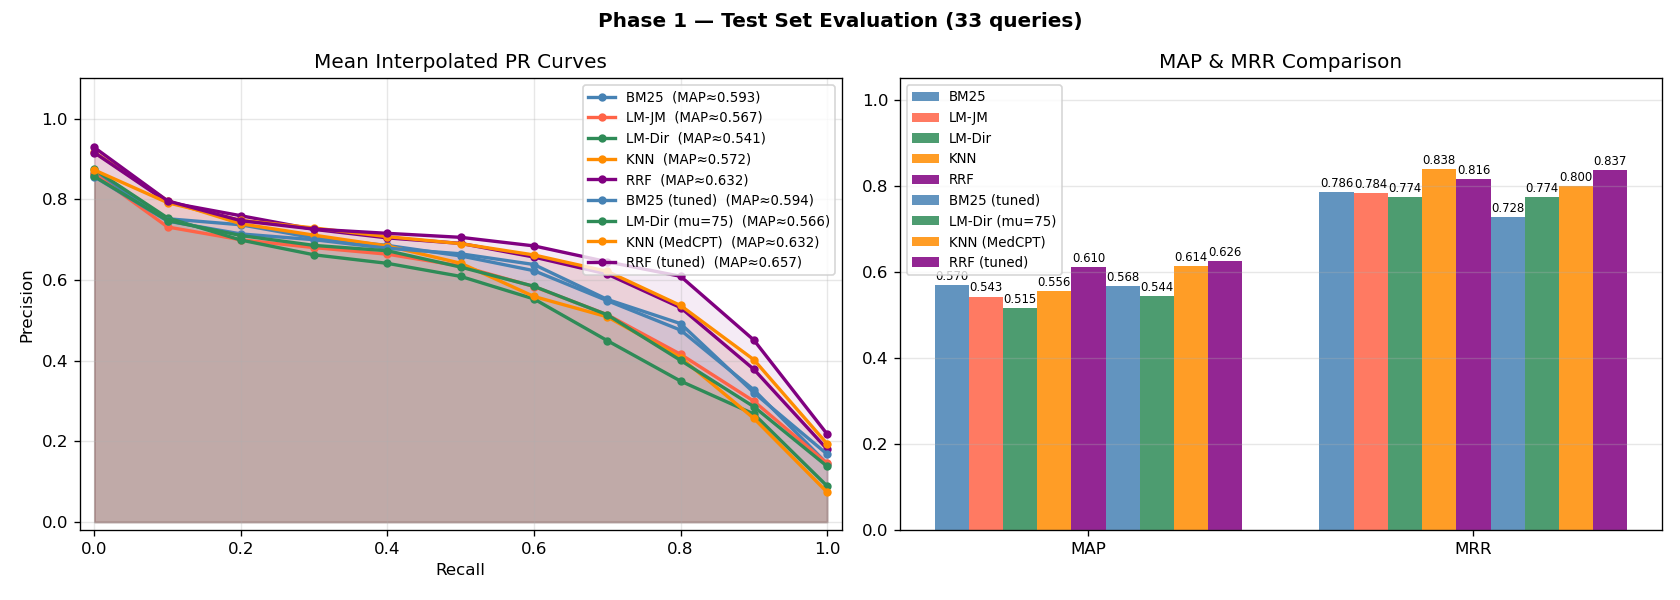
\includegraphics[width=\linewidth]{images/pr_curves.png}
  \caption{Mean interpolated PR curves for all strategies on the 33-query
           test set (left) with MAP/MRR bar chart (right). RRF (tuned) and
           KNN (MedCPT) dominate across the full recall range. LM variants
           show steeper early-recall drops.}
  \label{fig:pr_curves}
\end{figure}


%% Section 4: Conclusions
%%%%%%%%%%%%%%%%%%%%%%%%%%%%%%%%%%%%%%%%%%%%%%%%%
%%%%              CONCLUSIONS                %%%%
%%%%%%%%%%%%%%%%%%%%%%%%%%%%%%%%%%%%%%%%%%%%%%%%%

\section{Conclusions}
\label{sec:conclusions}

% ── 4a  ACHIEVEMENTS ──────────────────────────────────────────────────────────
\subsection{Phase 1 Achievements}
\label{sec:achievements}

We delivered a complete, modular IR pipeline on schedule (deadline Apr~13),
covering corpus loading, indexing, query building, retrieval, evaluation,
and result serialisation — all Colab-compatible.%
\footnote{Phase~1 notebook:
\url{https://colab.research.google.com/drive/1UvDhFXYEzZxse6gknDyBSUaq0EAHZkFV?usp=sharing}.}
Five retrieval strategies were implemented and compared: BM25,
LM-Jelinek-Mercer, LM-Dirichlet, dense KNN, and RRF fusion, following a
disciplined tuning protocol — query field ablation first, then 5-fold
cross-validation per strategy, with the test set touched exactly once.

The most impactful single design choice was selecting the MedCPT encoder,
which yielded $\Delta$NDCG@100 = +0.0501 on the test set
($0.7576 \to 0.8077$ versus the msmarco baseline; +0.0825 on 5-fold CV).
The locked Phase~2 strategy, KNN\,(MedCPT), reaches
NDCG@100 = 0.8077, MAP = 0.6143, and R@100 = 0.8933 on 33 test
topics; RRF (BM25+MedCPT, $k = 60$) pushes NDCG@100 to 0.8245 on the
same set.
The high Recall@100 of 0.8933 ensures a strong evidence pool for Phase~2
generation.

Several architectural decisions contributed to these results.
Our multi-field index design materialises every parameter configuration as a
dedicated OpenSearch field, enabling instant replay and side-by-side
comparison without re-encoding.
A systematic pooling-mode analysis (CLS vs.\ mean vs.\ mean-no-special)
established that architecture-appropriate pooling is critical before
comparing encoder families.
The exhaustive RRF sweep over 9~strategy pairs and 3~$k$ values confirmed
that sparse+dense fusion (BM25+KNN) is consistently the best pairing,
exploiting complementary lexical and semantic signals.
Finally, dual qrel scales (binary and graded) allowed evaluation with both
precision-oriented (MAP) and gain-discounted (NDCG) metrics, while the
robust odd/even topic split ensured no information leakage between selection
and final evaluation.

% ── 4b  LIMITATIONS ───────────────────────────────────────────────────────────
\subsection{Limitations}
\label{sec:limitations}

Several limitations should be noted.  The relevance judgements are derived
from automated BioGen submissions rather than human assessors, so systematic
biases are possible.  Moreover, the mean of 46.1 relevant documents per topic
is $3\text{--}15\times$ above standard TREC collections, which inflates MAP
and recall figures and makes them not directly comparable to published
benchmarks.  The 33-topic test set is relatively small, and the
fixed odd/even split offers no cross-validation guarantee that topic
difficulty is perfectly balanced.  A handful of relevant PMIDs referenced in
the qrels are absent from the 4{,}194-abstract corpus, creating an
irreducible recall ceiling.

Additionally, while the encoder comparison used brute-force cosine to control
for approximation noise, production KNN retrieval still relies on HNSW
indexing, which introduces some recall loss.

\subsection*{Future Work}

Phase~2 will add cross-encoder reranking with the
MedCPT-Cross-Encoder, LLM-augmented generation via vLLM with automatic
citation grounding, and LLM-as-judge evaluation.
Phase~3 will introduce a ReAct-style agentic loop — with Planner, Explorer,
Aggregator, and Report Writer roles — for multi-step reasoning over the
retrieval backbone.
Beyond the project scope, promising directions include learned sparse
retrieval (SPLADE) and late interaction (ColBERT) for higher recall at lower
rank cutoffs, as well as obtaining human relevance assessments to validate
the automated qrel quality.



%% -- Bibliography -----------------------------------------------
\bibliographystyle{splncs04}          % LNCS bibliography style
\bibliography{sections/references}    % points to sections/references.bib

\end{document}
